\documentclass[
11pt, % The default document font size, options: 10pt, 11pt, 12pt
%codirector, % Uncomment to add a codirector to the title page
]{charter} 


% El títulos de la memoria, se usa en la carátula y se puede usar el cualquier lugar del documento con el comando \ttitle
\titulo{Desarrollo de un sistema embebido para la gestión y monitoreo de cultivos verticales} 

% Nombre del posgrado, se usa en la carátula y se puede usar el cualquier lugar del documento con el comando \degreename
\posgrado{Carrera de Especialización en Sistemas Embebidos} 
%\posgrado{Carrera de Especialización en Internet de las Cosas} 
%\posgrado{Carrera de Especialización en Inteligencia Artificial}
%\posgrado{Maestría en Sistemas Embebidos} 
%\posgrado{Maestría en Internet de las cosas}
% IMPORTANTE: no omitir titulaciones ni tildación en los nombres, también se recomienda escribir los nombres completos (tal cual los tienen en su documento)
% Tu nombre, se puede usar el cualquier lugar del documento con el comando \authorname
\autor{Ing. José Luis Krüger }

% El nombre del director y co-director, se puede usar el cualquier lugar del documento con el comando \supname y \cosupname y \pertesupname y \pertecosupname
\director{Esp. Ing. Mariano Campos }
\pertenenciaDirector{FIUBA } 
\codirector{} % para que aparezca en la portada se debe descomentar la opción codirector en los parámetros de documentclass
\pertenenciaCoDirector{}

% Nombre del cliente, quien va a aprobar los resultados del proyecto, se puede usar con el comando \clientename y \empclientename
\cliente{Lic. Rocío Altamirano }
\empresaCliente{Particular }
 
\fechaINICIO{20 de agosto de 2024}		%Fecha de inicio de la cursada de GdP \fechaInicioName
\fechaFINALPlan{8 de octubre de 2024} 	%Fecha de final de cursada de GdP
\fechaFINALTrabajo{julio de 2025}	%Fecha de defensa pública del trabajo final


\begin{document}

\maketitle
\thispagestyle{empty}
\pagebreak


\thispagestyle{empty}
{\setlength{\parskip}{0pt}
\tableofcontents{}
}
\pagebreak


\section*{Registros de cambios}
\label{sec:registro}


\begin{table}[ht]
\label{tab:registro}
\centering
\begin{tabularx}{\linewidth}{@{}|c|X|c|@{}}
\hline
\rowcolor[HTML]{C0C0C0} 
Revisión & \multicolumn{1}{c|}{\cellcolor[HTML]{C0C0C0}Detalles de los cambios realizados} & Fecha      \\ \hline
0      & Creación del documento                                 &\fechaInicioName \\ \hline
1      & Se completa hasta el punto 5 inclusive                & {3} de {septiembre} de 2024 \\ \hline
2      & Se completa hasta el punto 9 inclusive					& {10} de {septiembre} de 2024 \\
\hline
3      & Se completa hasta el punto 12 inclusive					& {17} de {septiembre} de 2024 \\
\hline
4      & Se completa hasta el punto 15 inclusive					& {24} de {septiembre} de 2024 \\
\hline
%		  Se puede agregar algo más \newline
%		  En distintas líneas \newline
%		  Así                                                    & {día} de {mes} de 202X \\ \hline
%3      & Se completa hasta el punto 12 inclusive                & {día} de {mes} de 202X \\ \hline
%4      & Se completa el plan	                                 & {día} de {mes} de 202X \\ \hline

% Si hay más correcciones pasada la versión 4 también se deben especificar acá

\end{tabularx}
\end{table}

\pagebreak



\section*{Acta de constitución del proyecto}
\label{sec:acta}

\begin{flushright}
Buenos Aires, \fechaInicioName
\end{flushright}

\vspace{2cm}

Por medio de la presente se acuerda con el \authorname\hspace{1px} que su Trabajo Final de la \degreename\hspace{1px} se titulará ``\ttitle'' y consistirá en la implementación de un prototipo de un sistema de monitoreo y gestión de cultivo hidropónico. El trabajo tendrá un presupuesto preliminar estimado de 644 horas y un costo estimado de \$ 8 523 913, con fecha de inicio el \fechaInicioName\hspace{1px} y fecha de presentación pública en \fechaFinalName.

Se adjunta a esta acta la planificación inicial.

\vfill

% Esta parte se construye sola con la información que hayan cargado en el preámbulo del documento y no debe modificarla
\begin{table}[ht]
\centering
\begin{tabular}{ccc}
\begin{tabular}[c]{@{}c@{}}Dr. Ing. Ariel Lutenberg \\ Director posgrado FIUBA\end{tabular} & \hspace{2cm} & \begin{tabular}[c]{@{}c@{}}\clientename \\ \empclientename \end{tabular} \vspace{2.5cm} \\ 
\multicolumn{3}{c}{\begin{tabular}[c]{@{}c@{}} \supname \\ Director del Trabajo Final\end{tabular}} \vspace{2.5cm} \\
\end{tabular}
\end{table}




\section{1. Descripción técnica-conceptual del proyecto a realizar}
\label{sec:descripcion}

%\begin{consigna}{red} % El bloque "consigna" se usa para poner texto en rojo y dar una pequeña ayuda sobre cómo completar la sección. En cada entrega parcial deben eliminar los comandos begin y end del bloque consigna de las secciones que hayan completado.
%El objetivo es que el lector, en una o dos páginas, exponga de qué se trata el proyecto y cuáles son sus desafíos, cuál es la motivación para realizarlo y su importancia.

%Se debe introducir el contexto del proyecto, el estado del arte en la temática, describir la propuesta de valor, cuál es el problema que atiende y cuál es la solución que se propone. Se debe dar una descripción funcional de la solución que incluya un diagrama en bloques.

%Puede ser útil incluir en esta sección la respuesta a alguna de estas preguntas:

%\begin{itemize}
%	\item ¿Cuál es el contexto del proyecto, es un emprendimiento personal, un proyecto para una empresa, es parte del programa de vinculación con empresas del posgrado?
%	\item ¿Existen o aplican condiciones especiales al proyecto, financiamiento de algún programa público o privado, acuerdos de confidencialidad, acuerdos sobre la propiedad intelectual de los entregables u otros?
%	\item ¿Cómo se compara la solución propuesta con el estado del arte en el campo de aplicación? ¿En qué aspectos destaca?
%	\item ¿Ayuda a la explicación si se incluye un lienzo Canvas del Modelo de Negocio?
%	\item ¿En qué estado del ciclo de vida está la solución que se propone?
%	\item ¿Cuáles son las características del cliente (el adoptante de los entregables del proyecto) qué valora, qué necesita?
%	\item ¿Por dónde pasa la innovación?
%\end{itemize}

%La descripción técnica-conceptual \textbf{debe incluir al menos un diagrama en bloques del sistema} y descripción funcional de la solución propuesta.

%Las figuras se deben mencionar en el texto ANTES de que aparezcan con una frase como la siguiente: ``En la figura \ref{fig:diagBloques} se presenta el diagrama en bloques del sistema. Se observa que...''.  La regla es que las figuras nunca pueden ir antes de ser mencionadas en el texto, porque sino el lector no entiende por qué de pronto aparece una figura.

%\begin{figure}[htpb]
%\centering 
%\includegraphics[width=.65\textwidth]{./Figuras/diagBloques.png}
%\caption{Diagrama en bloques del sistema.}
%\label{fig:diagBloques}
%\end{figure}

%\vspace{25px}

%El tamaño del texto en TODAS las figuras debe ser adecuado \textbf{para que NO pase lo que ocurre en la figura \ref{fig:diagBloques}}, donde el lector debe esforzarse para poder leer el texto. 

%Los colores usados en el diagrama deben ser adecuados, tal que ayuden a comprender mejor el diagrama. Se recomienda evitar colores primarios (como rojo, verde o cyan) y usar la gama de colores pastel.
%\end{consigna}

Con la población mundial que ronda los 8000 millones de personas y sigue en crecimiento, la agricultura enfrenta el reto de ser más eficiente y sostenible. Los cultivos verticales se presentan como una solución innovadora que optimiza el uso del espacio y los recursos, especialmente en entornos urbanos donde el suelo es limitado y costoso.

Este tipo de agricultura utiliza técnicas como la hidroponía, que permite un uso preciso del agua, y la aeroponía, que maximiza el oxígeno disponible para las raíces. Además, las granjas verticales aprovechan áreas infrautilizadas, como edificios abandonados o naves industriales, y permiten cultivar alimentos en zonas donde la agricultura tradicional resulta dificil de desarrollar. Así, se logra una mayor densidad de cultivo y se contribuye a la sostenibilidad al reducir el uso de pesticidas y fertilizantes.

Aunque los cultivos verticales requieren un alto nivel de tecnología y tienen costes energéticos asociados, su capacidad para ahorrar recursos, disminuir la huella de carbono y fomentar la producción local y el autoconsumo los posiciona como una opción clave para la agricultura del futuro.

Como proyecto final de la especialización en sistemas embebidos, se propone desarrollar un sistema de monitoreo y gestión para cultivos verticales. Dicho trabajo se trata de un emprendimiento personal y tiene por objetivo permitir controlar y potenciar los factores de crecimiento de las plantas como la nutrición del sustrato, la luz necesaria para fotosíntesis o la oxigenación de las raíces y, al mismo tiempo, optimizar el uso de un recurso tan preciado como el agua.

Por un lado, para lograr  la optimización del agua, se utilizará un circuito cerrado de modo que el desperdicio del recurso sea mínimo. Por otro, el monitoreo y control de variables como el pH de la solución nutritiva, su conductividad, temperatura, etc. permitirá lograr un óptimo crecimiento de las plantas al mismo tiempo que el usuario será alertado de cualquier anomalía que se produzca en el sistema.

Los sistemas hidropónicos actuales dependen del usuario para medir de forma manual variables clave como el pH y la temperatura, o directamente no se miden. Utilizan temporizadores genéricos para el riego y, en muchos casos, no se controla la temperatura o la iluminación que reciben las plantas, lo que limita su eficiencia en comparación con los métodos tradicionales. La solución que se presenta en este informe, en cambio, no solo permite medir con precisión todas estas variables, sino que también ajusta automáticamente los controles necesarios, con minima intervención del usuario. Esto aporta trazabilidad y facilita el ajuste de parámetros para mejorar la productividad a futuro.

\begin{figure}[htpb]
\centering 
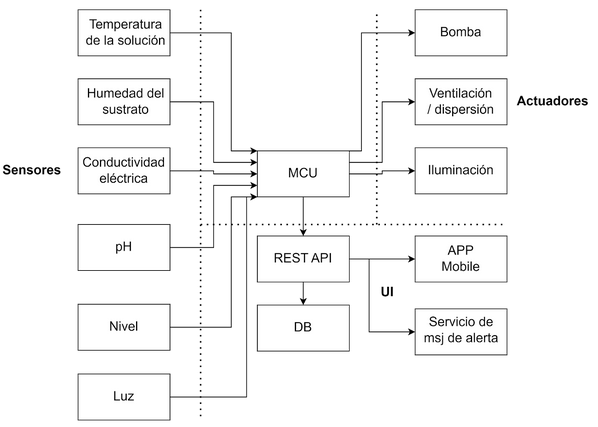
\includegraphics[width=.85\textwidth]{./Figuras/d_bloques.png}
\caption{Diagrama en bloques del sistema.}
\label{fig:d_bloques}
\end{figure}

En la figura \ref{fig:d_bloques} se presenta el diagrama en bloques de la solución propuesta. Este sistema permitirá controlar el riego, la iluminación y la oxigenación de las raíces, al tiempo que monitoreará otras variables críticas para su operación. Se diseñará para un cultivo urbano pequeño, ubicado en el interior de una vivienda, pero será fácilmente escalable, ya que se podrá ampliar simplemente multiplicando el módulo completo. 
%El servidor central será diseñado para gestionar y centralizar la información de una gran cantidad de módulos, de modo que el usuario solo necesite registrar el suyo en el sistema.

\section{2. Identificación y análisis de los interesados}
\label{sec:interesados}

%\begin{consigna}{red} % este comando se debe borrar para la entrega, junto con la contraparte \end{consigna}{red} 

\begin{table}[ht]
%\caption{Identificación de los interesados}
%\label{tab:interesados}
\begin{tabularx}{\linewidth}{@{}|l|X|X|l|@{}}
\hline
\rowcolor[HTML]{C0C0C0} 
Rol           & Nombre y Apellido & Organización 	& Puesto 	\\ \hline
Cliente       & \clientename      &\empclientename	&     -   	\\ \hline
Responsable   & \authorname       &    FIUBA   		& Alumno 	\\ \hline
Orientador    & \supname	      & \pertesupname	& Director del Trabajo Final \\ \hline
Usuario final &  Agricultor orgánico   	  &    -          	&   -     	\\ \hline
\end{tabularx}
\end{table}


\begin{itemize}
	\item Orientador: El \supname será quien dirija técnicamente el proyecto.

	\item Cliente: La \clientename será quien testee y valide el prototipo del proyecto.
\end{itemize}

%\end{consigna} % este comando se debe borrar para la entrega, junto con la contraparte \begin{consigna}{red}


\section{3. Propósito del proyecto}
\label{sec:proposito}

Desarrollar un prototipo funcional y escalable que permita automatizar y optimizar los sistemas hidropónicos actuales, de modo que el usuario no necesite realizar monitoreos y ajustes manuales. Busca mejorar la eficiencia en el uso de recursos como el agua, los nutrientes y la energía, además de garantizar un control preciso de las condiciones de cultivo. Con esto, se espera aumentar la productividad y la sostenibilidad de los cultivos hidropónicos mediante un sistema que ofrece trazabilidad completa y facilita la toma de decisiones para futuros ajustes, logrando una producción más rentable, sustentable y tolerante a cambios en las condiciones ambientales.
\section{4. Alcance del proyecto}
\label{sec:alcance}

%\begin{consigna}{red}
%¿Qué se incluye y que no se incluye en este proyecto?

%Se refiere al trabajo que se va a hacer para entregar el producto o resultado especificado. 

%Explicitar todo lo quede comprendido dentro del alcance del proyecto. Por ejemplo:

El proyecto incluye:
\begin{itemize}
	\item Desarrollo del prototipo funcional y escalable.
		\begin{itemize}
		\item Diseño de un sistema automatizado para el control del riego, la iluminación y la oxigenación en cultivos hidropónicos verticales.
		\item Desarrollo del firmware para el microcontrolador.
		%\item Desarrollo de una aplicación REST API (incluida la base de datos) y una PWA (Progressive Web App) como interfaz de usuario.
		\item Desarrollo de una aplicación web como interfaz de usuario.
		\end{itemize}
	\item Pruebas y validación del prototipo.
		\begin{itemize}
		\item Realización de pruebas en un entorno controlado con cultivos hidropónicos verticales para validar la precisión y efectividad del sistema en el control del riego, la iluminación y la oxigenación.
		\item Ajuste de componentes y firmware según los resultados obtenidos durante las pruebas.
		\end{itemize}
	\item Desarrollo de la PCB centralizadora de los módulos electrónicos utilizados.
	\item Memoria técnica.
	
\end{itemize}

El proyecto no incluye:
\begin{itemize}
	\item Control de otras variables ambientales, como el pH o la temperatura del sustrato.
	\item Soporte técnico o mantenimiento continuado del sistema después de la entrega del prototipo.
	\item Adaptación del sistema a otros tipos de cultivos hidropónicos no verticales o infraestructuras específicas que no sean verticales.
	\item Producción a gran escala del sistema automatizado, más allá del prototipo desarrollado.
	\item Desarrollo de sistemas de seguridad adicionales más allá de lo necesario para el prototipo.
	\item Implementación de tecnología para la optimización del consumo energético para producción a gran escala.
	\item Desarrollo de una aplicación REST API (incluida la base de datos).
	\item Procesamiento estadístico de los datos almacenados.
	
\end{itemize}

%Explicitar además todo lo que no quede incluido (``El presente proyecto no incluye...'')

%\end{consigna}


\section{5. Supuestos del proyecto}
\label{sec:supuestos}

%\begin{consigna}{red}
%``Para el desarrollo del presente proyecto se supone que: ...''

\begin{itemize}
	\item Se dispondrá del apoyo de un director con el conocimiento necesario para orientar técnicamente el proyecto y guiar el desarrollo del prototipo.
	\item Se dispondrá de todos los materiales necesarios, incluidos sensores, actuadores, controladores y otros componentes electrónicos para el desarrollo del prototipo.
	\item La integración de los sistemas de riego, iluminación y ventilación con el software desarrollado será viable técnicamente y no presentará incompatibilidades significativas.
	\item  Se contará con el tiempo suficiente para completar todas las fases del proyecto, desde el diseño y desarrollo hasta las pruebas y ajustes necesarios, sin retrasos significativos.
	\item Existirá un entorno controlado y adecuado para la instalación y prueba del prototipo en condiciones similares a las de operación real para cultivos hidropónicos verticales.
	\item Las condiciones macroeconómicas permanecerán estables, sin variaciones significativas en el costo de materiales o componentes.
	\item El PCB podrá desarrollarse.
\end{itemize}

%Por ejemplo, se podrían incluir supuestos respecto a disponibilidad de tiempo y recursos humanos y materiales, sobre la factibilidad técnica de distintos aspectos del proyecto, sobre otras cuestiones que sean necesarias para el éxito del proyecto como condiciones macroeconómicas o reglamentarias.
%\end{consigna}

\section{6. Requerimientos}
\label{sec:requerimientos}

%\begin{consigna}{red}
%Los requerimientos deben enumerarse y de ser posible estar agrupados por afinidad, por ejemplo:

\begin{enumerate}
	\item \textbf{Requerimientos funcionales:}
\begin{enumerate}
    \item El prototipo debe permitir el control automático del riego, iluminación y oxigenación del cultivo, garantizando que el tiempo de respuesta para cambios en el ambiente no supere los 5 segundos (prioridad alta).
    
    \item El sistema debe monitorear variables ambientales relevantes como temperatura (rango de - 15 a 50 °C, precisión de ±1 °C), humedad del sustrato (rango de 0\% a 100\%, precisión de ±3\%), nivel de la solución nutritiva (mínimo 3/4 de la altura total del contenedor), conductividad eléctrica (rango de 1 a 4 mS/cm, precisión de ±0.1 mS/cm), y pH (rango de 5.5 a 7.5, precisión de ±0.1) (prioridad alta).
    
    \item El usuario debe poder activar o desactivar manualmente las secuencias de riego mediante la interfaz gráfica, con un tiempo de respuesta menor a 2 segundos (prioridad media).
     
    %\item El sistema debe ser escalable, permitiendo la conexión y control de hasta 50 módulos hidropónicos sin degradar el tiempo de respuesta, que deberá mantenerse inferior a 10 segundos para cada módulo adicional (prioridad media).
    
    \item El firmware debe incluir un servidor embebido para la gestión local y remota de los parámetros del sistema, con disponibilidad 24/7 (prioridad alta).
    
    \item El usuario debe poder configurar el sistema mediante una interfaz gráfica amigable, accesible desde un dispositivo móvil (Android/iOS) a través de la red Wi-Fi, con tiempos de carga inferiores a 5 segundos (prioridad alta).
    
    \item El producto debe permitir la programación de secuencias de riego en base a fecha, hora y duración o humedad del sustrato, con una precisión de ±1 minuto en la ejecución de las secuencias (prioridad alta).
    
\end{enumerate}

	\item \textbf{Requerimientos de documentación:}
		\begin{enumerate}
			\item Se debe proporcionar un manual de usuario detallado con instrucciones de configuración y operación del sistema (prioridad baja).
			\item Se deben realizar diagramas esquemáticos del circuito, PCB y diagramas de conexiones (prioridad media).
			\item El proyecto debe incluir documentación del código fuente con comentarios claros y comprensibles (prioridad media).
		\end{enumerate}
	\item \textbf{Requerimiento de testing:}
	\begin{enumerate}
	\item El sistema debe ser sometido a pruebas de funcionalidad completas para verificar el correcto funcionamiento de todas las características (prioridad alta).
	\item Se deben realizar pruebas de estrés para garantizar la estabilidad del sistema bajo condiciones extremas de operación (prioridad media).
	\item El firmware debe pasar por pruebas de validación de comunicación de red (HTTP o MQTT) (prioridad alta).
	\item El hardware debe ser testeado para asegurar su resistencia y fiabilidad en ambientes urbanos interiores y exteriores (prioridad alta).
	\end{enumerate}
	\item \textbf{Requerimientos de la interfaz de usuario:}
	\begin{enumerate}
	\item La interfaz de usuario debe ser intuitiva y fácil de usar, con menús claros para la configuración de parámetros del control del cultivo (prioridad alta).
	\item La interfaz debe mostrar el estado en tiempo real de todas las variables monitoreadas (temperatura, humedad, nivel de agua, etc.) (prioridad alta).
	%\item La interfaz debe permitir el registro y gestión de múltiples módulos hidropónicos (prioridad baja).
	\item La interfaz debe ser responsiva y compatible con dispositivos móviles modernos (prioridad alta).
	\end{enumerate}
	\item \textbf{Requerimientos interoperabilidad:}
	\begin{enumerate}
	\item Se debe asegurar compatibilidad con un protocolo de comunicación estándar como HTTP o MQTT (prioridad alta).
	\end{enumerate}
	\item \textbf{Requerimientos de normativas y regulaciones:}
	\begin{enumerate}
	\item El diseño del hardware debe cumplir con las normativas de seguridad eléctrica establecidas por la resolución 169/2018 de la Secretaría de Comercio, que adopta la norma IEC 62368-1 para equipos eléctricos (prioridad alta).
	\item  Se debe cumplir con las regulaciones de radiofrecuencia y comunicaciones establecidas por la Enacom (Ente Nacional de Comunicaciones), que incluye la homologación de equipos bajo las normas de la Resolución 197/2004 y sus modificaciones (prioridad alta).
	\item El hardware debe cumplir con las normas de compatibilidad electromagnética conforme a la Resolución 92/98 de la Secretaría de Industria, que adopta normas internacionales como la IEC CISPR 22 para la emisión de interferencias electromagnéticas (prioridad alta).
	\end{enumerate}
	\item \textbf{Requerimientos opcionales:}
	\begin{enumerate}
	    \item El servidor podría generar alarmas y notificaciones en caso de condiciones anómalas, como fallos de sensores o nivel crítico de solución nutritiva (menor al 10\% del volumen total), con un tiempo de notificación menor a 1 minuto desde la detección.
       \item El servidor central podría almacenar y procesar los datos de todos los módulos conectados, permitiendo trazabilidad y análisis histórico.
	\item El firmware podría permitir la integración con plataformas de automatización del hogar (e.g., Home Assistant, Google Home).
	\item El sistema podría ser capaz de exportar datos en formatos compatibles con aplicaciones de análisis de datos (CSV, JSON).
	\item El sistema podría incluir una funcionalidad de análisis predictivo para optimizar las secuencias de riego basadas en datos históricos.
	\item La interfaz podría incluir un módulo de visualización de datos avanzado para el análisis gráfico de la eficiencia del cultivo.
	\item Podría añadirse un control PID de temperatura de la solución nutritiva.
	\end{enumerate}
\end{enumerate}

%Leyendo los requerimientos se debe poder interpretar cómo será el proyecto y su funcionalidad.

%Indicar claramente cuál es la prioridad entre los distintos requerimientos y si hay requerimientos opcionales. 

%\textbf{¡¡¡No olvidarse de que los requerimientos incluyen a las regulaciones y normas vigentes!!!}

%Y al escribirlos seguir las siguientes reglas:
%\begin{itemize}
%	\item Ser breve y conciso (nadie lee cosas largas). 
%	\item Ser específico: no dejar lugar a confusiones.
%	\item Expresar los requerimientos en términos que sean cuantificables y medibles.
%\end{itemize}

%\end{consigna}

\section{7. Historias de usuarios (\textit{Product backlog})}
\label{sec:backlog}

%\begin{consigna}{red}
%Descripción: en esta sección se deben incluir las historias de usuarios y su ponderación (\textit{history points}). Recordar que las historias de usuarios son descripciones cortas y simples de una característica contada desde la perspectiva de la persona que desea la nueva capacidad, generalmente un usuario o cliente del sistema. La ponderación es un número entero que representa el tamaño de la historia comparada con otras historias de similar tipo.

%Se debe indicar explícitamente el criterio para calcular los \textit{story points} de cada historia.

%El formato propuesto es: 
%\begin{enumerate}
%\item ``Como [rol] quiero [tal cosa] para [tal otra cosa]."
%\item ``Como usuario quiero poder cultivar vegetales de forma particular en mi propio domicilio, un departamento ubicado en un 8vo piso. Por esta razón, no cuento con el espacio necesario para el cultivo en tierra."
%\item ``No cuento con el tiempo necesario para dedicarle al cuidado de las plantas, por lo que el sistema debería poder funcionar con la minima participación de alguien."
%\item ``Me gustaría poder cambiar de lugar el cultivo cuando lo crea conveniente."

%\textit{Story points}: 8 (complejidad: 3, dificultad: 2, incertidumbre: 3)
%\end{enumerate}
%end{consigna}

La ponderación de cada historia de usuario se basa en la serie de Fibonacci y se clasifica en tres niveles:

\begin{itemize}
    \item Baja (1)
    \item Media (3)
    \item Alta (5)
\end{itemize}

El puntaje total de cada historia se redondea hacia arriba al valor más cercano en la serie de Fibonacci, asegurando que los Story Points reflejen adecuadamente la magnitud del trabajo requerido.


%\begin{itemize}
\textbf{Historia 1:} ``Como agricultor urbano, quiero que el sistema hidropónico se encargue del riego, la luz y la oxigenación, así puedo cultivar sin preocuparme por hacer ajustes todo el tiempo."

        \begin{itemize}
            \item \textbf{Complejidad:} Alta (5)
            \item \textbf{Dificultad:} Media (3)
            \item \textbf{Incertidumbre:} Alta (5)
        \end{itemize}
        \textit{\textbf{Story Points:}} 13
    %\end{itemize}

\textbf{Historia 2:} ``Como alguien que vive en un departamento, quiero poder cultivar mis propias verduras en casa, aunque no tenga jardín."

        \begin{itemize}
            \item \textbf{Complejidad:} Media (3)
            \item \textbf{Dificultad:} Baja (1)
            \item \textbf{Incertidumbre:} Media (3)
        \end{itemize}
        \textit{\textbf{Story Points:}} 8
    %\end{itemize}

\textbf{Historia 3:} ``Como usuario ocupado, quiero que el sistema sea lo más autónomo posible, así no tengo que estar pendiente de las plantas todos los días."

        \begin{itemize}
            \item \textbf{Complejidad:} Baja (1)
            \item \textbf{Dificultad:} Baja (1)
            \item \textbf{Incertidumbre:} Baja (1)
        \end{itemize}
        \textit{\textbf{Story Points:}} 3

\textbf{Historia 4:} ``Como alguien que se muda con frecuencia, quiero que el cultivo sea fácil de trasladar para poder llevarlo conmigo a diferentes lugares."

        \begin{itemize}
            \item \textbf{Complejidad:} Media (3)
            \item \textbf{Dificultad:} Media (3)
            \item \textbf{Incertidumbre:} Media (3)
        \end{itemize}
        \textit{\textbf{Story Points:}} 13

 \textbf{Historia 5:} ``Como usuario preocupado por mis plantas, quiero recibir notificaciones en mi celular si algo anda mal, como falta de agua o nutrientes, para poder arreglarlo a tiempo."

        \begin{itemize}
            \item \textbf{Complejidad:} Alta (5)
            \item \textbf{Dificultad:} Media (3)
            \item \textbf{Incertidumbre:} Media (3)
        \end{itemize}
        \textit{\textbf{Story Points:}} 13

 \textbf{Historia 6:} ``Como aficionado a la hidroponía, quiero ajustar los parámetros de riego, luz y nutrientes según lo que necesiten mis cultivos, para lograr los mejores resultados."

        \begin{itemize}
            \item \textbf{Complejidad:} Alta (5)
            \item \textbf{Dificultad:} Alta (5)
            \item \textbf{Incertidumbre:} Media (3)
        \end{itemize}
       \textit{\textbf{Story Points:}} 13

 \textbf{Historia 7:} ``Como investigador de cultivos urbanos, quiero tener acceso a los datos históricos del cultivo para analizar cómo mejorar la producción."

        \begin{itemize}
            \item \textbf{Complejidad:} Media (3)
            \item \textbf{Dificultad:} Media (3)
            \item \textbf{Incertidumbre:} Baja (1)
        \end{itemize}
        \textit{\textbf{Story Points:}} 8
  
%\end{itemize}

\section{8. Entregables principales del proyecto}
\label{sec:entregables}

%\begin{consigna}{red}
Los entregables del proyecto son:

\begin{itemize}
	\item Manual de usuario.
	%\item Diagrama de circuitos esquemáticos.
	%\item Código fuente del firmware.
	%\item Diagrama de instalación.
	\item Prototipo funcional.
	\item Memoria del trabajo final.
	%\item etc...
\end{itemize}
%\end{consigna}

\section{9. Desglose del trabajo en tareas}
\label{sec:wbs}

%\begin{consigna}{red}
%El WBS debe tener relación directa o indirecta con los requerimientos.  Son todas las actividades que se harán en el proyecto para dar cumplimiento a los requerimientos. Se recomienda mostrar el WBS mediante una lista indexada:

A continuación se realiza el desglose del proyecto en tareas:

\begin{enumerate}
\item Planificación del proyecto (40 h):
	\begin{enumerate}
	\item Realizar la arquitectura general del proyecto (15 h).
	\item Realizar el plan del proyecto (25 h).
	\end{enumerate}
\item Investigación (50 h):
	\begin{enumerate}
	\item Estudiar el funcionamiento del ESP32 y los sensores (20 h).
	\item Investigación sobre hidroponía y requerimientos del sistema físico (30 h).
	\end{enumerate}
\item Diseño del sistema (50 h):
	\begin{enumerate}
	\item Diseño de la arquitectura general del sistema (30 h).
	%\item Diseño de la base de datos (8 h).
	%\item Diseño del servidor central (20 h).
	\item Diseño del módulo de control del prototipo (20 h).
	\end{enumerate}
\item Desarrollo del sistema hidropónico (30 h):
	\begin{enumerate}
	\item Adquisición de un sistema hidropónico vertical estándar (2 h).
	\item Instalación de los componentes del sistema de riego, iluminación y oxigenación (20 h).
	\item Pruebas iniciales del sistema hidropónico (8 h).
	\end{enumerate}
\item Desarrollo del hardware (70 h):
	\begin{enumerate}
	\item Diseño del circuito y simulación (15 h).
	\item Diseño de la PCB (15 h).
	\item Fabricación de la PCB (5 h).
	\item Inspección de la PCB (5 h).
	\item Montaje de componentes en la PCB (15 h).
	\item Pruebas de validación del hardware (15 h).
	\end{enumerate}
\item Desarrollo del firmware (145 h):
	\begin{enumerate}
	\item Desarrollo del software para control de riego (15 h).
	\item Desarrollo del software para control de iluminación (15 h).
	\item Desarrollo del software para control de oxigenación (15 h).
	\item Desarrollo de \textit{drivers} para los dispositivos implicados (20 h).
	\item Implementación del sistema operativo para el módulo de control (20 h).
	\item Desarrollo del servidor embebido en el módulo de control (40 h).
	\item Implementación del protocolo de comunicación HTTP o MQTT (20 h).
	\end{enumerate}
\item Desarrollo de la interfaz de usuario (39 h):
	\begin{enumerate}
	\item Maquetado de la interfaz de usuario minimalista para el control del sistema (8 h).
	\item Desarrollo de la interfaz gráfica de usuario (GUI) minimalista para dispositivos móviles y/o web (16 h).
	\item Pruebas de usabilidad y ajustes en la interfaz (15 h).
	\end{enumerate}
%\item Desarrollo del servidor central (40 h):
	%\begin{enumerate}
	%\item Desarrollo del software del servidor central (20 h).
	%\item Integración del servidor con los módulos de control (10 h).
	%\item Desarrollo e integración del servicio de alarmas (10 h).
	%\end{enumerate}
\item Integración y pruebas (80 h):
	\begin{enumerate}
	\item Integración de módulos en el prototipo funcional (30 h).
	\item Pruebas de integración y rendimiento del sistema (20 h).
	\item Pruebas de comunicación y control centralizado (15 h).
	\item Validación final del sistema completo (15 h).
	\end{enumerate}
\item Documentación y entrega (140 h):
	\begin{enumerate}
	\item Elaboración de documentación técnica del sistema (40 h).
	\item Elaboración de memoria técnica (40 h).
	\item Preparación del manual de usuario (40 h).
	\item Presentación de resultados y entrega del proyecto (20 h).
	\end{enumerate}
\end{enumerate}

Cantidad total de horas: 644 h.

%\textbf{¡Importante!:} la unidad de horas es h y va separada por espacio del número. Es incorrecto escribir ``23hs".

%\textbf{Se recomienda que no haya ninguna tarea que lleve más de 40 h.} De ser así se recomienda dividirla en tareas de menor duración.

%\end{consigna}

\section{10. Diagrama de Activity On Node}
\label{sec:AoN}

%\begin{consigna}{red}
%Armar el AoN a partir del WBS definido en la etapa anterior.

%Una herramienta simple para desarrollar los diagramas es el Draw.io (\url{https://app.diagrams.net/}).
%\href{https://app.diagrams.net}{Draw.io}


\begin{figure}[htpb]
\centering 
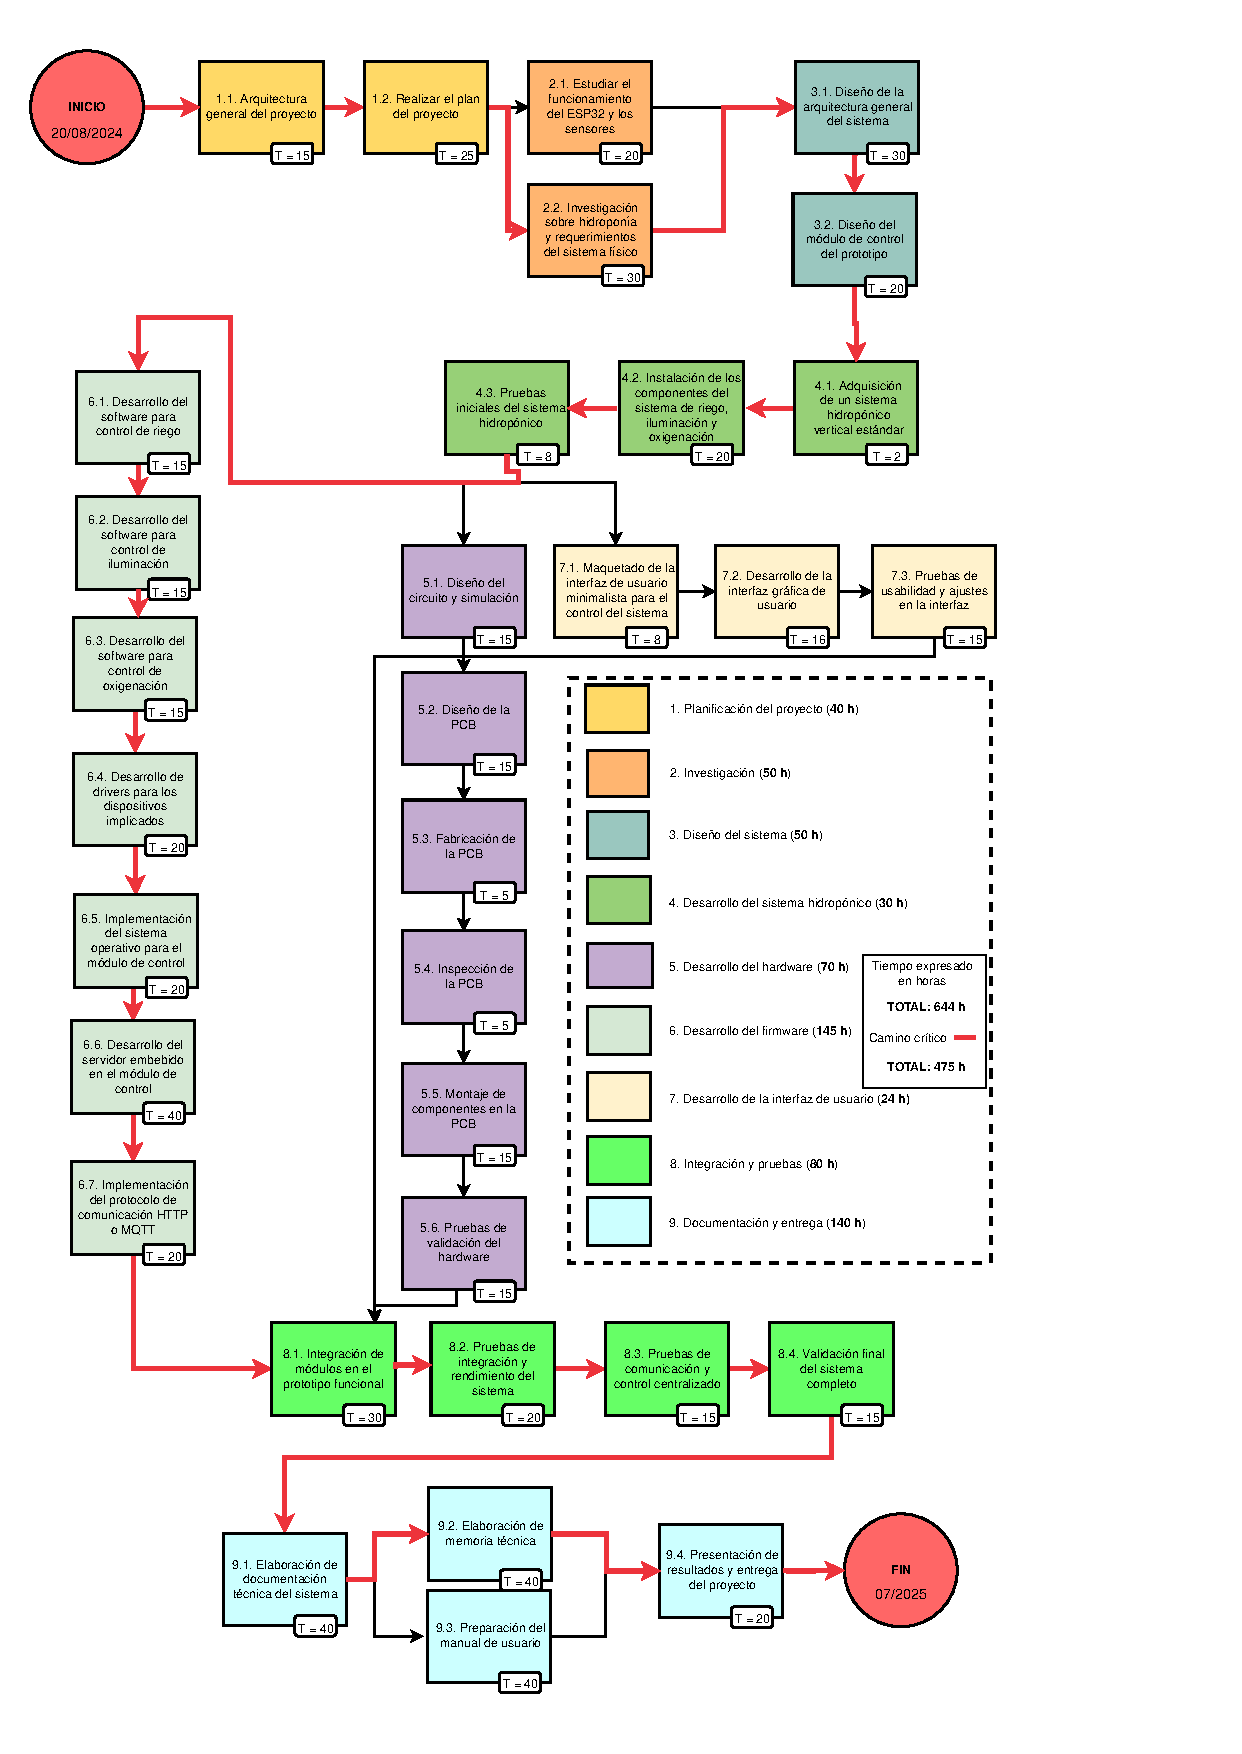
\includegraphics[width=1.0\textwidth]{./Figuras/AoN.pdf}
\caption{Diagrama de \textit{Activity on Node}.}
\label{fig:AoN}
\end{figure}

%Indicar claramente en qué unidades están expresados los tiempos.
%De ser necesario indicar los caminos semi críticos y analizar sus tiempos mediante un cuadro.
%Es recomendable usar colores y un cuadro indicativo describiendo qué representa cada color.

%\end{consigna}

\section{11. Diagrama de Gantt}
\label{sec:gantt}

Para el diagrama \textit{Gantt} se consideró una dedicación parcial de entre 3 y 4 horas todos los días
hábiles.

%\begin{consigna}{red}
%Existen muchos programas y recursos \textit{online} para hacer diagramas de Gantt, entre los cuales destacamos:

%\begin{itemize}
%\item Planner
%\item GanttProject
%\item Trello + \textit{plugins}. En el siguiente link hay un tutorial oficial: \\ \url{https://blog.trello.com/es/diagrama-de-gantt-de-un-proyecto}
%\item Creately, herramienta online colaborativa. \\\url{https://creately.com/diagram/example/ieb3p3ml/LaTeX}
%\item Se puede hacer en latex con el paquete \textit{pgfgantt}\\ \url{http://ctan.dcc.uchile.cl/graphics/pgf/contrib/pgfgantt/pgfgantt.pdf}
%\end{itemize}

%Pegar acá una captura de pantalla del diagrama de Gantt, cuidando que la letra sea suficientemente grande como para ser legible. 
%Si el diagrama queda demasiado ancho, se puede pegar primero la ``tabla'' del Gantt y luego pegar la parte del diagrama de barras del diagrama de Gantt.

%Configurar el software para que en la parte de la tabla muestre los códigos del EDT (WBS).\\
%Configurar el software para que al lado de cada barra muestre el nombre de cada tarea.\\
%Revisar que la fecha de finalización coincida con lo indicado en el Acta Constitutiva.

%En la figura \ref{fig:diagGantt}, se muestra un ejemplo de diagrama de gantt realizado con el paquete de \textit{pgfgantt}. 
%En la plantilla pueden ver el código que lo genera y usarlo de base para construir el propio.

%Las fechas pueden ser calculadas utilizando alguna de las herramientas antes citadas. Sin embargo, el siguiente ejemplo
%fue elaborado utilizando 
%\href{https://docs.google.com/spreadsheets/d/1fBz8NhSpc4tkkhz3KjJCbh1nR_ltDkfEcZi4tZXduqs}{esta hoja de cálculo}.

%Es importante destacar que el ancho del diagrama estará dado por la longitud del texto utilizado para las tareas 
%(Ejemplo: tarea 1, tarea 2, etcétera) y el valor \textit{x unit}. Para mejorar la apariencia del diagrama, es necesario
%ajustar este valor y, quizás, acortar los nombres de las tareas.

%\begin{figure}[htpb]
%  \begin{center}
%    \begin{ganttchart}[
%      time slot unit=day,
%      time slot format=isodate,
%      x unit=0.038cm,
%      y unit title=0.7cm,
%      y unit chart=0.6cm,
%      milestone/.append style={xscale=4}
%      ]{2021-03-05}{2021-12-16}
%      \gantttitlecalendar*{2021-03-05}{2021-12-16}{year} \\
%      \gantttitlecalendar*{2021-03-05}{2021-12-16}{month} \\
%      \ganttgroup{Duración Total}{2021-03-05}{2021-12-16} \\
      %%%%%%%%%%%%%%%%%Organización
%      \ganttgroup{Organización}{2021-03-05}{2021-04-16} \\
%      \ganttbar{Planificación del proyecto}{2021-03-05}{2021-04-15} \\
%      %%%%%%%%%%%%%%%%%Ejecución
%      \ganttgroup{Ejecución}{2021-04-16}{2021-10-21} \\
%      \ganttbar{Tarea 1}{2021-04-16}{2021-04-29} \\
%      \ganttbar{Tarea 2}{2021-04-30}{2021-05-13} \\
%      \ganttbar{Tarea 3}{2021-05-14}{2021-05-27} \\
%      \ganttbar{Tarea 4}{2021-05-28}{2021-07-12} \\
%      \ganttbar{Tarea 5}{2021-07-13}{2021-08-09} \\
%      \ganttbar{Tarea 6}{2021-08-10}{2021-09-23} \\
%      \ganttbar{Tarea 7}{2021-09-24}{2021-09-30} \\
%      \ganttbar{Tarea 8}{2021-10-01}{2021-10-14} \\
%      \ganttbar{Tarea 9}{2021-10-15}{2021-10-21} \\
      % %%%%%%%%%%%%%%%%%Finalización
%      \ganttgroup{Finalización}{2021-10-22}{2021-12-16} \\
%      \ganttbar{Memoria v1}{2021-10-22}{2021-11-04} \\
%      \ganttbar{Memoria v2}{2021-11-05}{2021-11-18} \\
%      \ganttbar{Memoria final}{2021-11-19}{2021-12-02} \\
%
      % La fecha del siguiente milestone es la fecha en que terminamos la memoria
%      \ganttmilestone{Enviar memoria al director}{2021-12-02} \\
%      \ganttbar{Elaborar la presentación}{2021-12-03}{2021-12-16} \\
%      \ganttmilestone{Ensayo de la presentación}{2021-12-16} \\
      %%%%%%%%%%%%%%%%%%%%%%%%%%%%%%%%%%%%%%%%%%%%%%%%%%%%%%%%%%%%%%%
%    \end{ganttchart}
%  \end{center}
%  \caption{Diagrama de gantt de ejemplo}
%  \label{fig:gantt}
%\end{figure}

\begin{figure}[htpb]
\centering 
%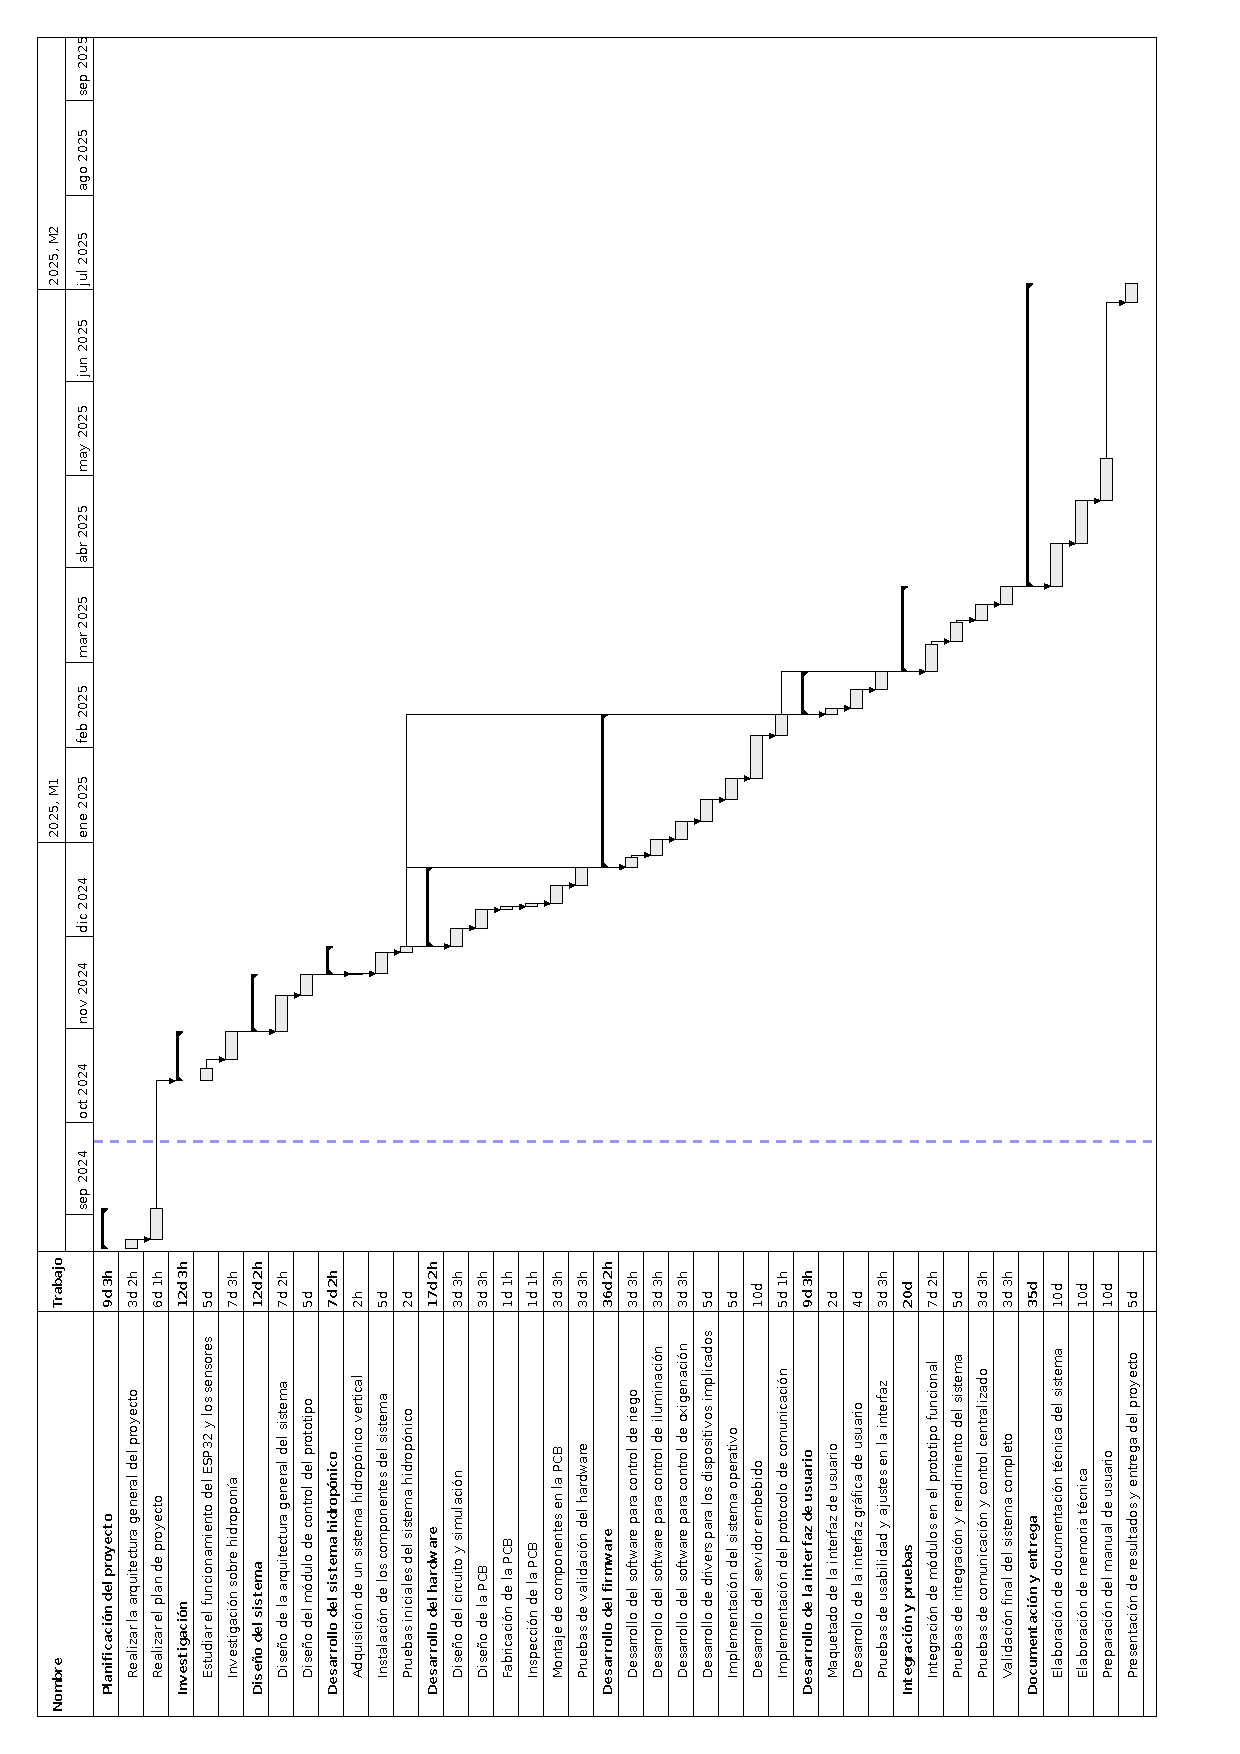
\includegraphics[height=.85\textheight]{./Figuras/salida.pdf}
%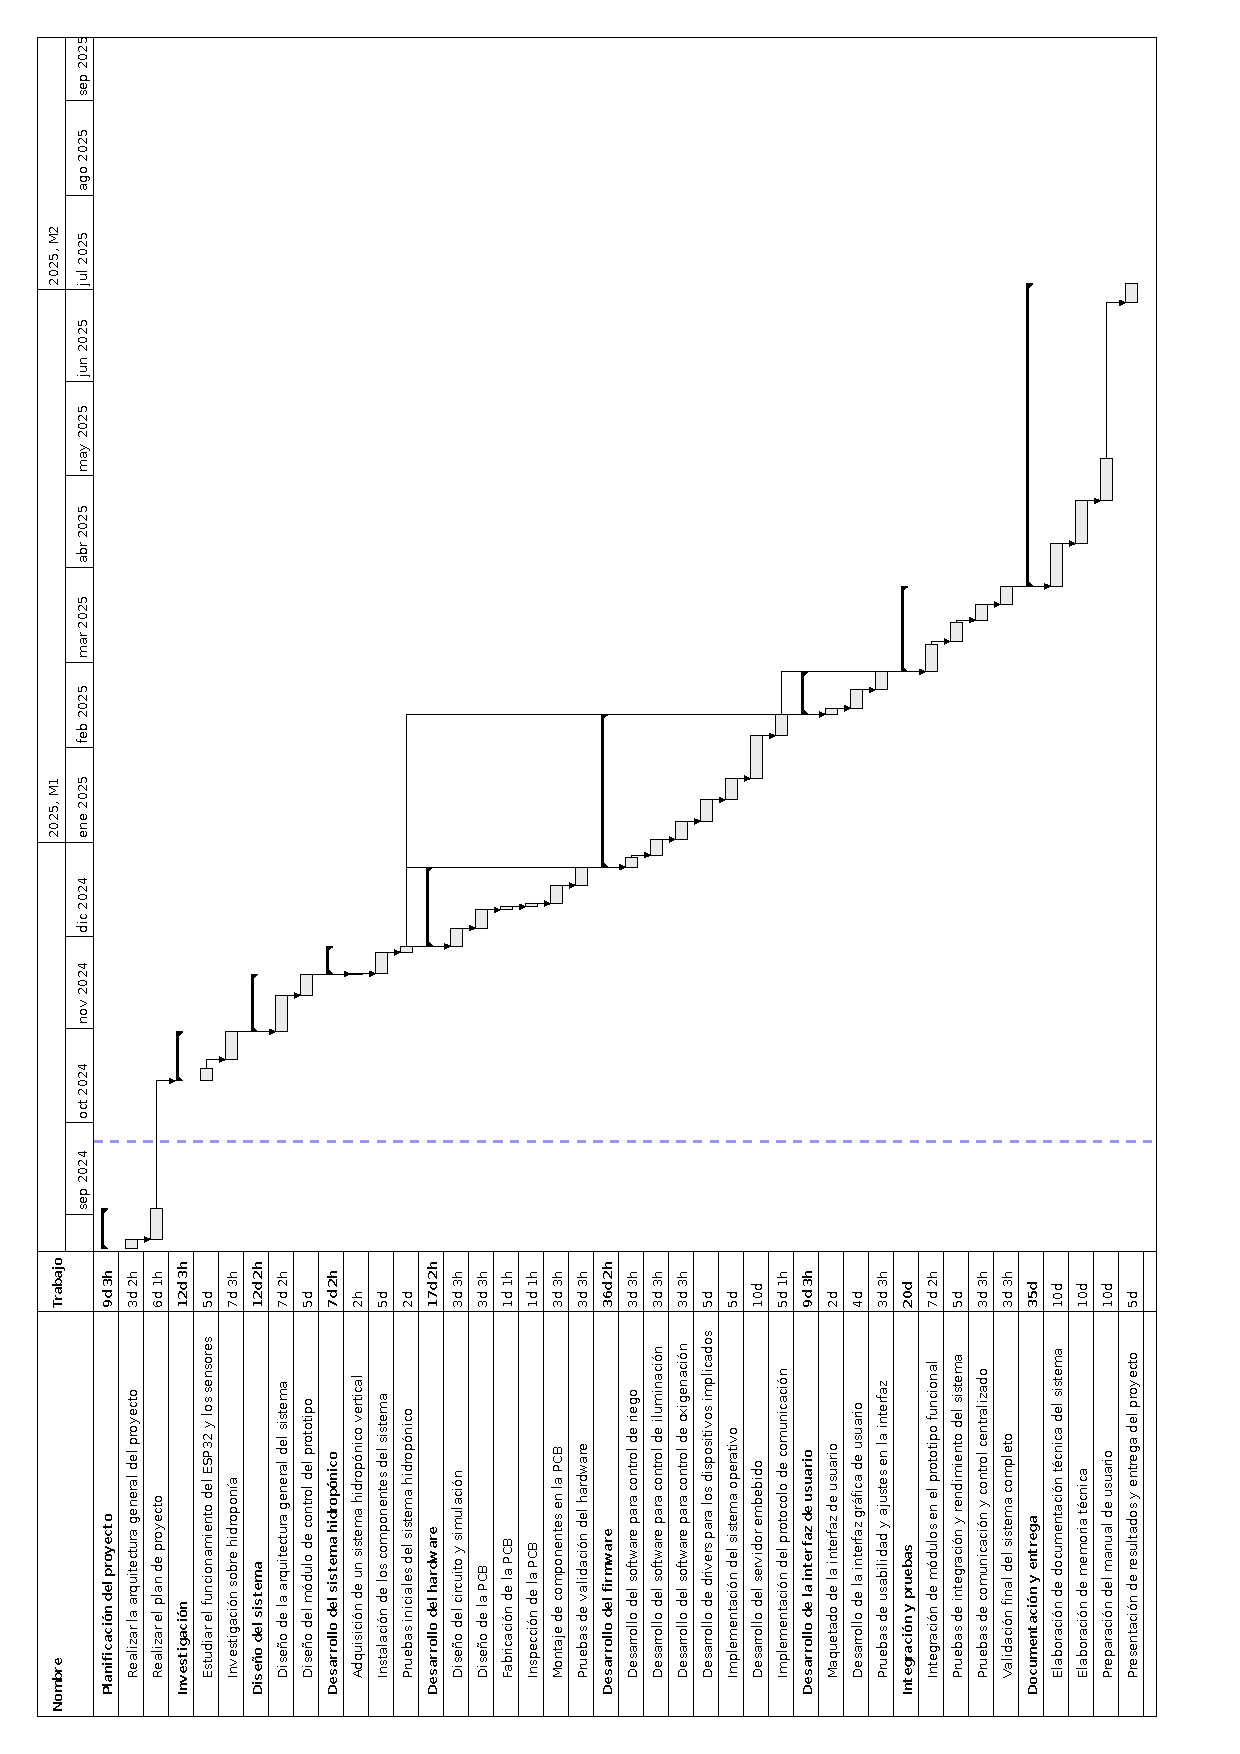
\includegraphics[width=\linewidth]{./Figuras/salida.pdf}
%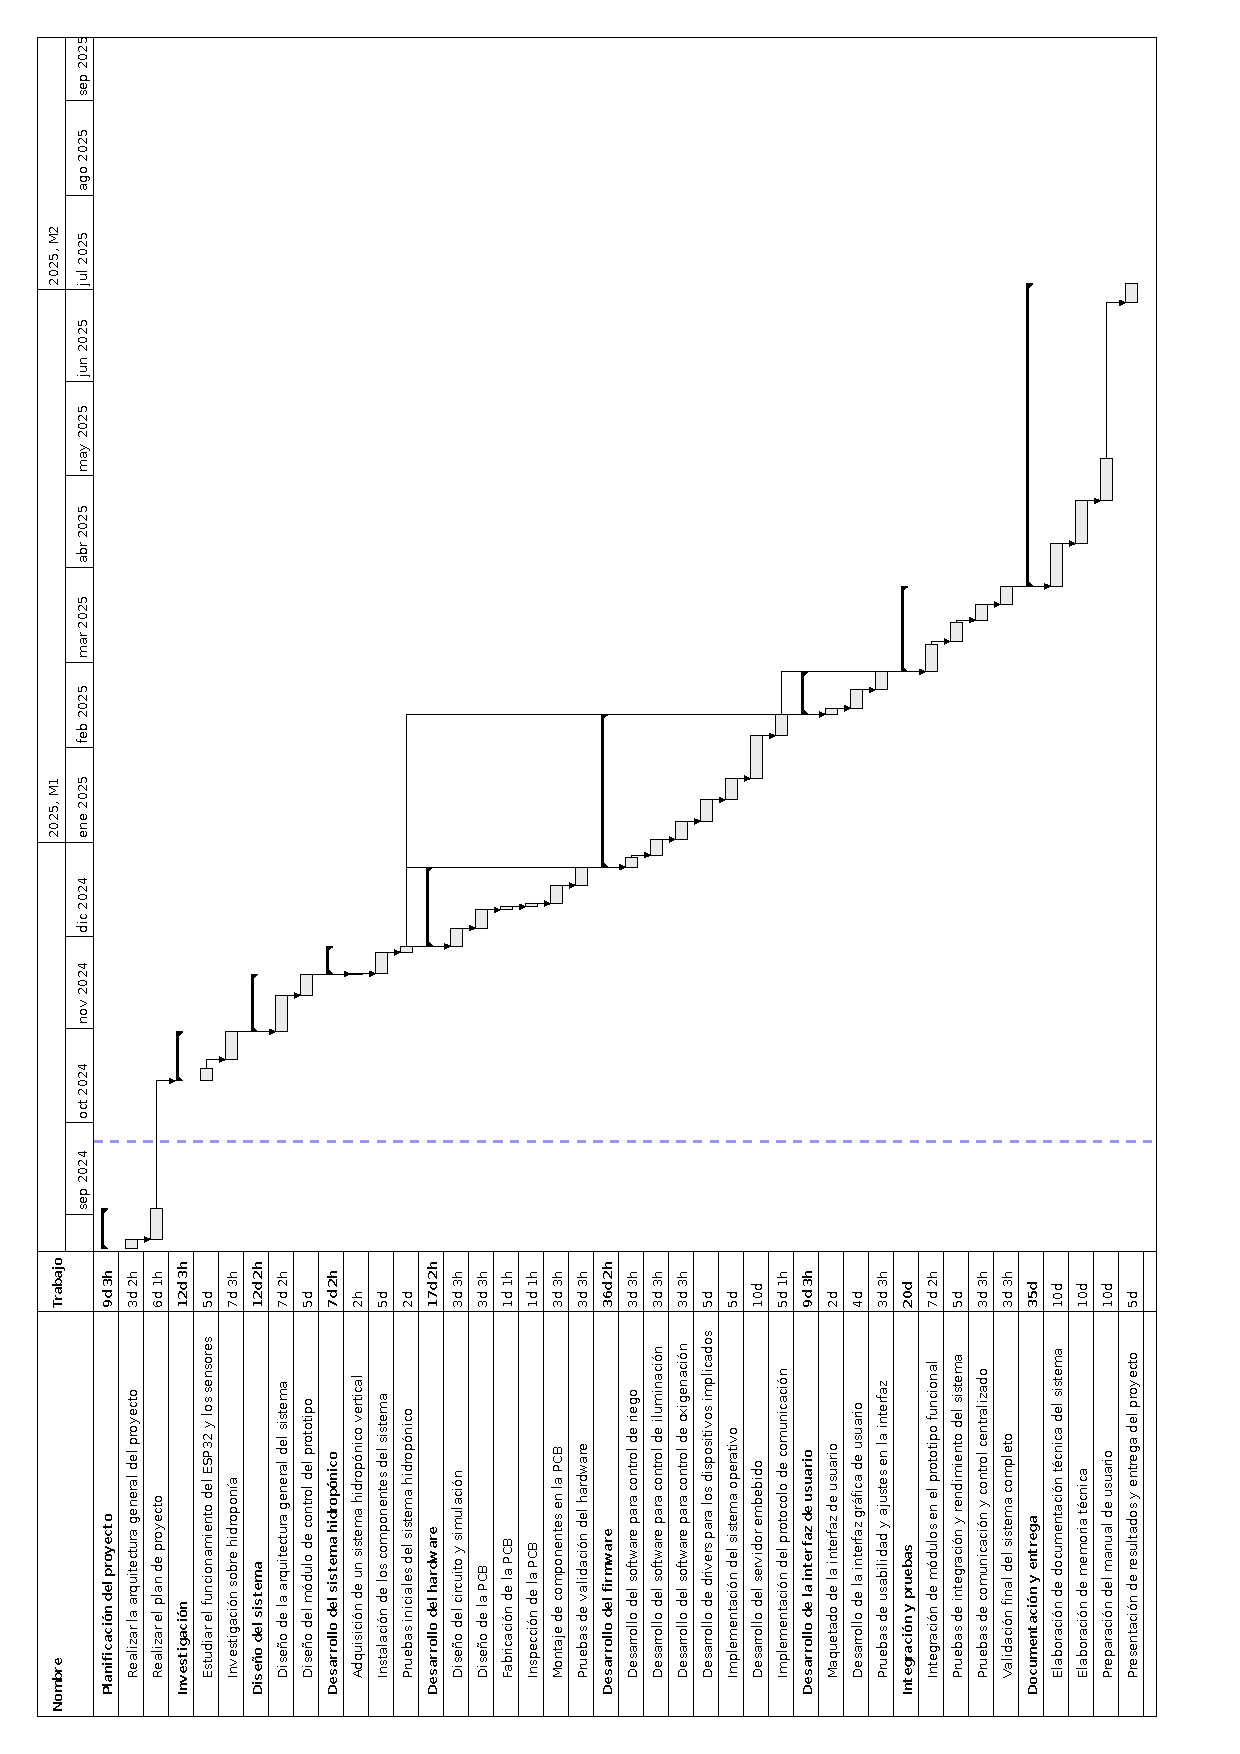
\includegraphics[width=\linewidth, height=0.95\linewidth]{./Figuras/salida.pdf}
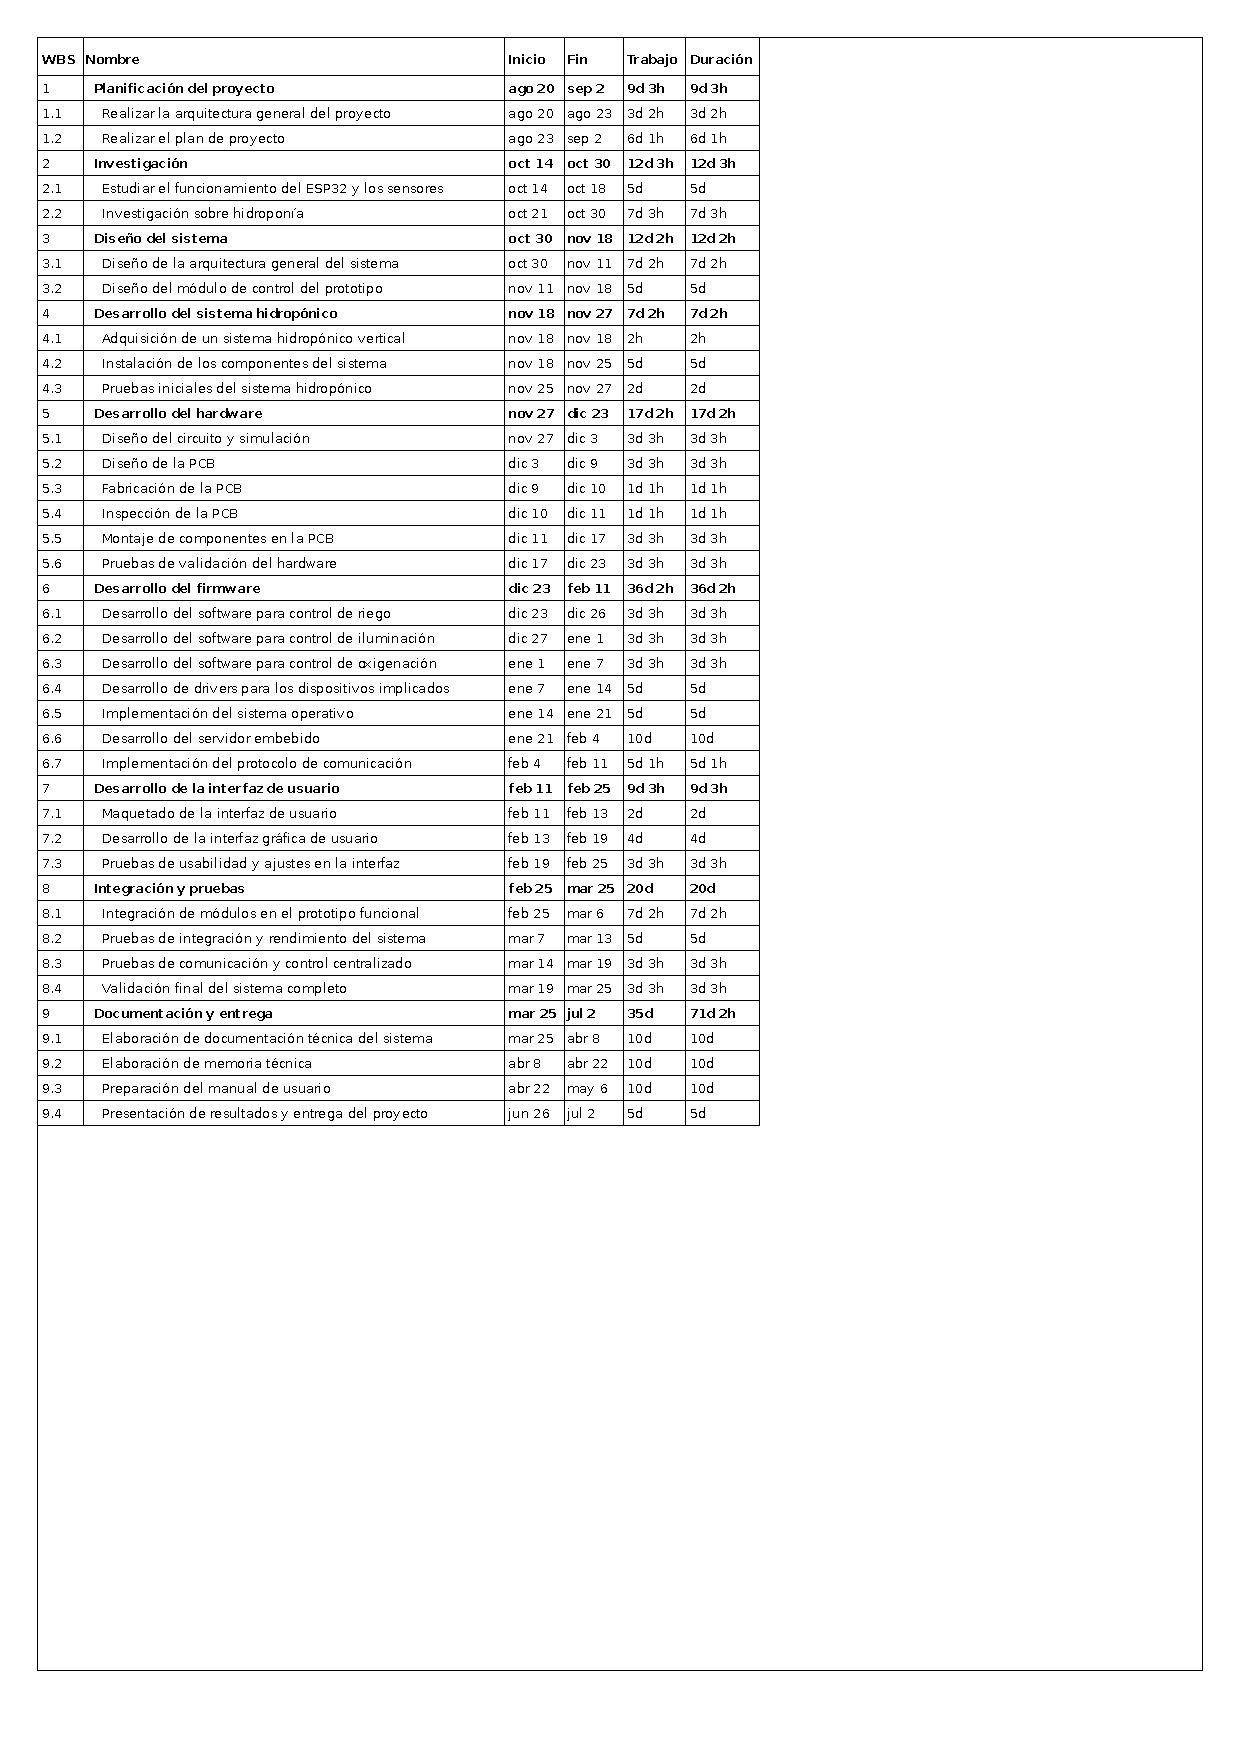
\includegraphics[trim=0 300 0 0, clip,width=\linewidth, height=0.97\textheight]{./Figuras/tareas.pdf}
\caption{Detalle de las tareas del diagrama \textit{Gantt}.} %Modificar este título acorde.
\label{fig:diagGantt}
\end{figure}

\begin{landscape}

\begin{figure}[htpb]
\centering
%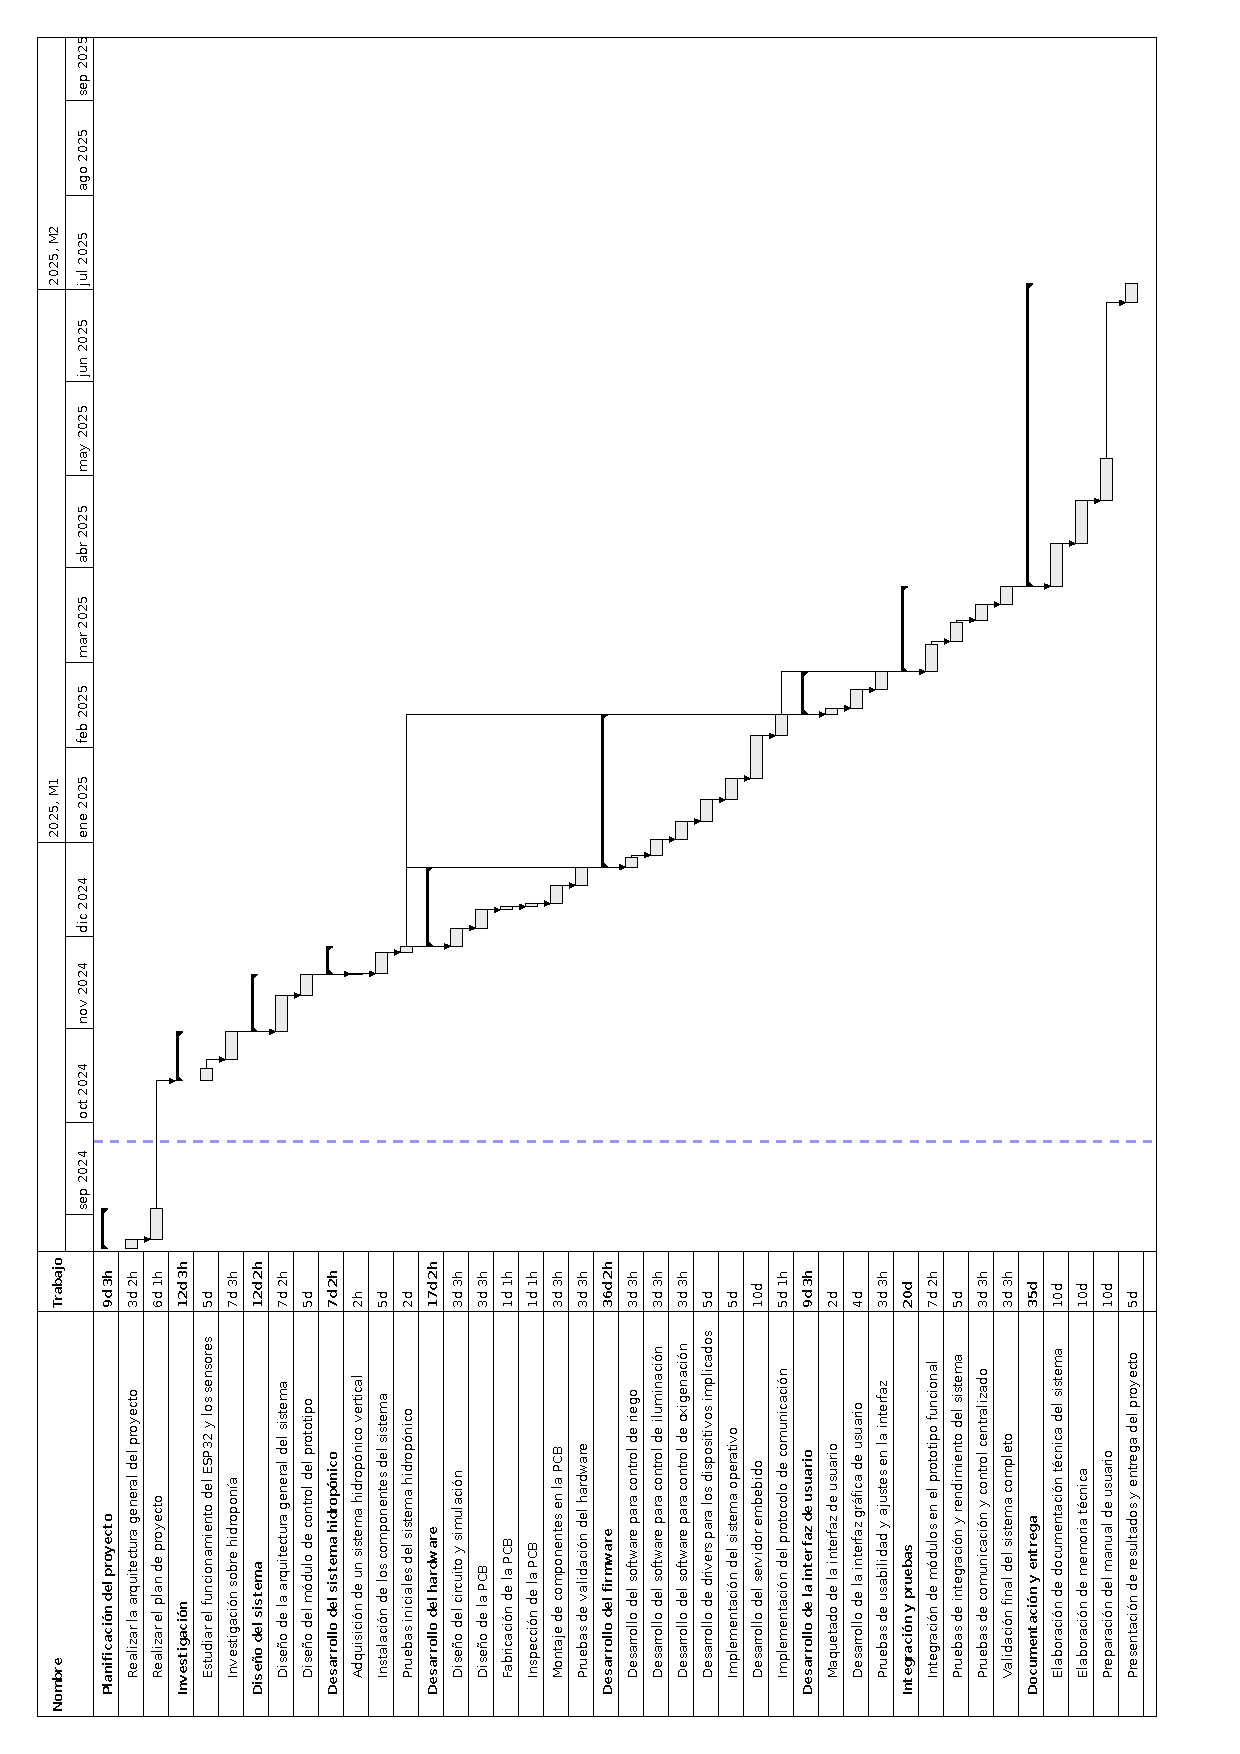
\includegraphics[trim=0 0 0 0, clip, width=\linewidth, height=0.97\textheight, angle=270]{./Figuras/salida.pdf}
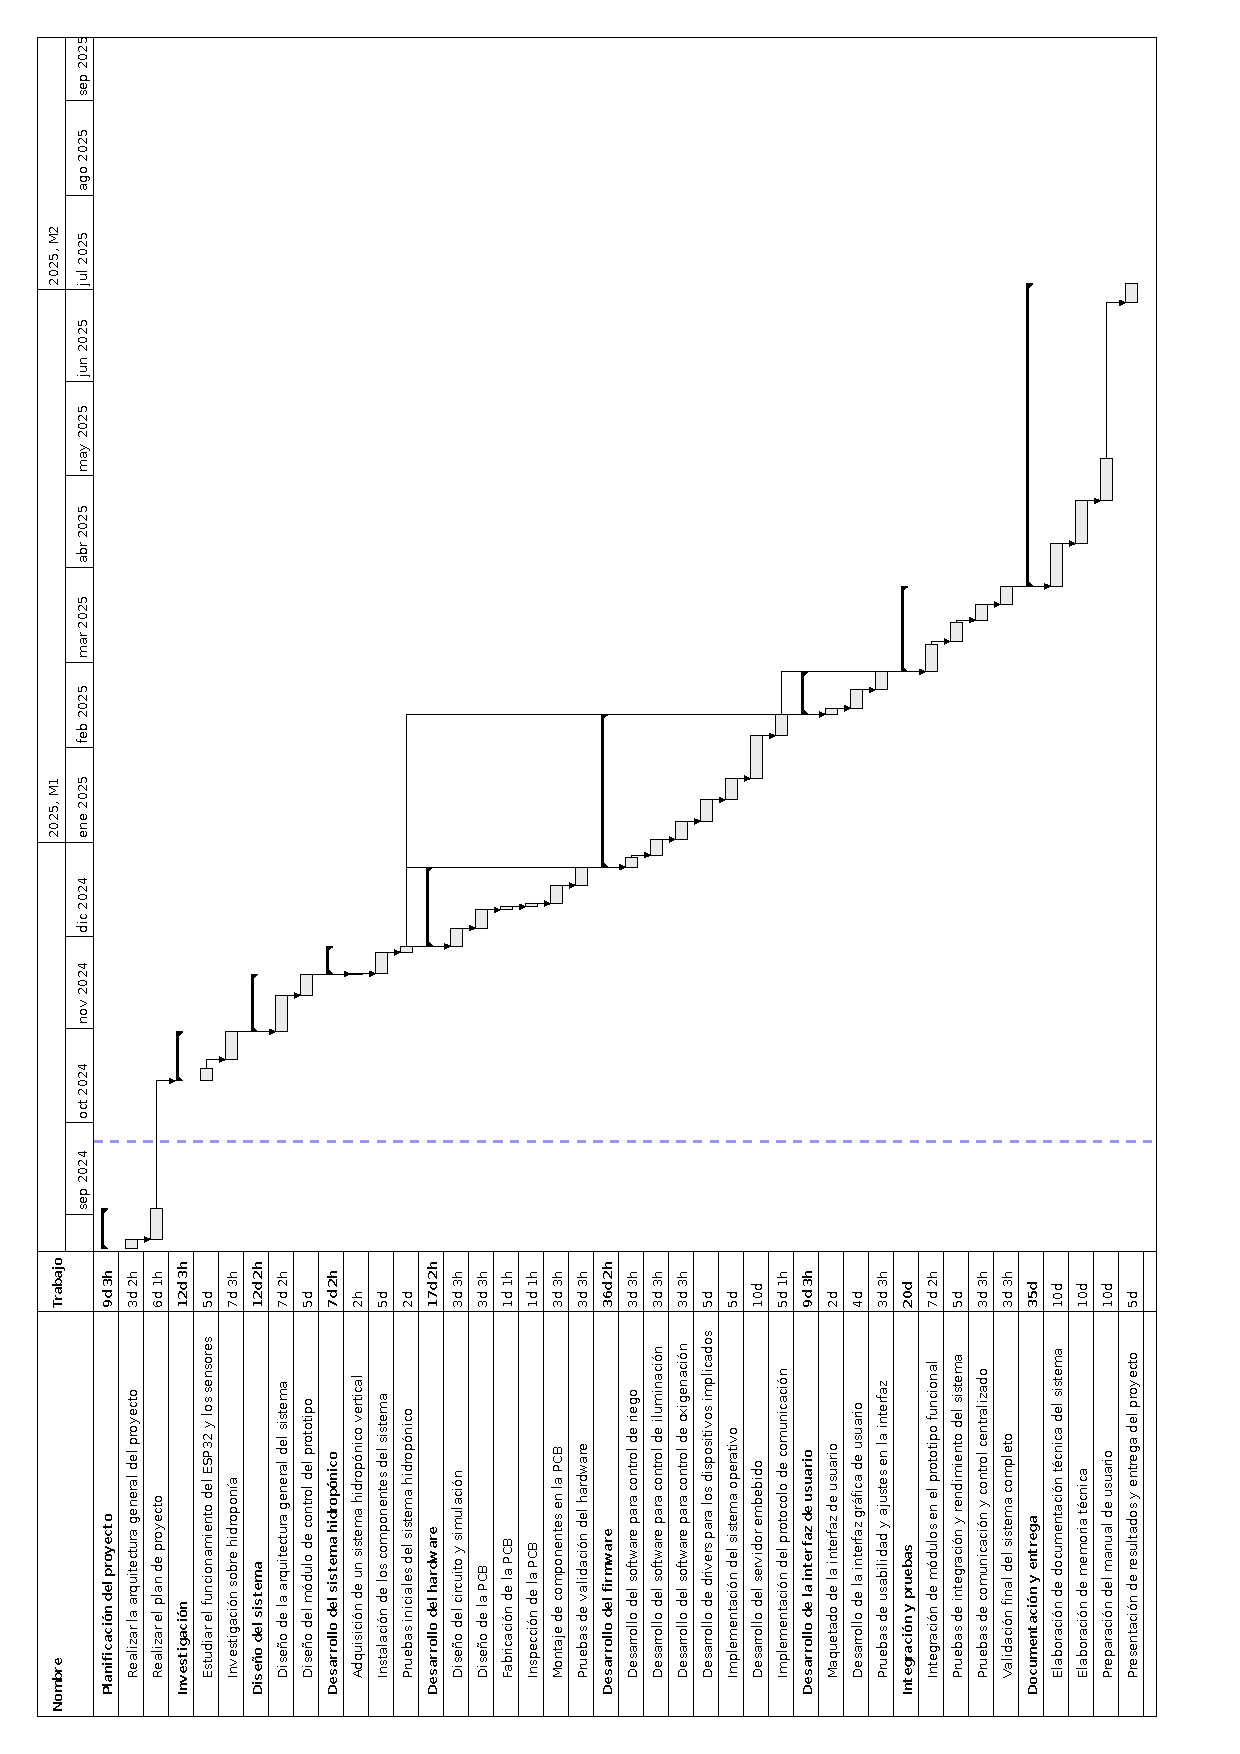
\includegraphics[angle=270, width=1.5\textheight]{./Figuras/salida.pdf}
\caption{Diagrama \textit{Gantt} desarrollado en Planner.} %Modificar este título acorde.
\label{fig:diagGantt}
\end{figure}


\end{landscape}

%\end{consigna}


\section{12. Presupuesto detallado del proyecto}
\label{sec:presupuesto}

%\begin{consigna}{red}
%Si el proyecto es complejo entonces separarlo en partes:
%\begin{itemize}
%	\item Un total global, indicando el subtotal acumulado por cada una de las áreas.
%	\item El desglose detallado del subtotal de cada una de las áreas.
%\end{itemize}

%IMPORTANTE: No olvidarse de considerar los COSTOS INDIRECTOS.

%Incluir la aclaración de si se emplea como moneda el peso argentino (ARS) o si se usa moneda extranjera (USD, EUR, etc). Si es en moneda extranjera se debe indicar la tasa de conversión respecto a la moneda local en una fecha dada.

%\end{consigna}

En el siguiente cuadro se muestra el detalle de los costos del proyecto expresados en pesos argentinos (ARS).

\begin{table}[htpb]
\centering
\begin{tabularx}{\linewidth}{@{}|X|c|r|r|@{}}
\hline
\rowcolor[HTML]{C0C0C0} 
\multicolumn{4}{|c|}{\cellcolor[HTML]{C0C0C0}COSTOS DIRECTOS} \\ \hline
\rowcolor[HTML]{C0C0C0} 
Descripción &
  \multicolumn{1}{c|}{\cellcolor[HTML]{C0C0C0}Cantidad} &
  \multicolumn{1}{c|}{\cellcolor[HTML]{C0C0C0}Valor unitario} &
  \multicolumn{1}{c|}{\cellcolor[HTML]{C0C0C0}Valor total} \\ \hline
ESP32S WROOM &
  \multicolumn{1}{c|}{01 u.} & 
  \multicolumn{1}{c|}{10 692} &
  \multicolumn{1}{c|}{10 692} \\ \hline
  
  Módulo sensor de luz con LDR &
  \multicolumn{1}{c|}{01 u.} & 
  \multicolumn{1}{c|}{2052} &
  \multicolumn{1}{c|}{2052} \\ \hline 
  
   Torre hidropónica vertical 22 macetas + bomba&
  \multicolumn{1}{c|}{01 u.} & 
  \multicolumn{1}{c|}{240 000} &
  \multicolumn{1}{c|}{240 000} \\ \hline
  
     Lámpara cultivo indoor Amnesia Cob 400w &
  \multicolumn{1}{c|}{01 u.} & 
  \multicolumn{1}{c|}{140 000} &
  \multicolumn{1}{c|}{140 000} \\ \hline
  
    Sensor de pH-4502c &
  \multicolumn{1}{c|}{01 u.} & 
  \multicolumn{1}{c|}{92 500} &
  \multicolumn{1}{c|}{92 500} \\ \hline

  DS18B20 &
  \multicolumn{1}{c|}{01 u.} & 
  \multicolumn{1}{c|}{2400} &
  \multicolumn{1}{c|}{2400} \\ \hline  
  
 Sensor de humedad C.&
  \multicolumn{1}{c|}{01 u.} &
  \multicolumn{1}{c|}{4500} &
  \multicolumn{1}{c|}{4500} \\ \hline
  
   Fuente de alimentación 5 VDC 2 A&
  \multicolumn{1}{c|}{01 u.} &
  \multicolumn{1}{c|}{7000} &
  \multicolumn{1}{c|}{7000} \\ \hline
  
     Cooler fan 220 V&
  \multicolumn{1}{c|}{01 u.} &
  \multicolumn{1}{c|}{10 000} &
  \multicolumn{1}{c|}{10 000} \\ \hline 
  
Módulo rele relay de 4 canales 5 V 10 A&
  \multicolumn{1}{c|}{01 u.} &
  \multicolumn{1}{c|}{8500} &
  \multicolumn{1}{c|}{8500} \\ \hline
  
  Módulo sensor de calidad de agua TDS + sonda analógica&
  \multicolumn{1}{c|}{01 u.} &
  \multicolumn{1}{c|}{30 000} &
  \multicolumn{1}{c|}{30 000} \\ \hline 
  
  Servicios profesionales &
  \multicolumn{1}{c|}{644 u.} & 
  \multicolumn{1}{c|}{12 000} &
  \multicolumn{1}{c|}{7 728 000} \\ \hline
  

\multicolumn{3}{|c|}{SUBTOTAL} &
  \multicolumn{1}{c|}{8 275 644} \\ \hline
\rowcolor[HTML]{C0C0C0} 
\multicolumn{4}{|c|}{\cellcolor[HTML]{C0C0C0}COSTOS INDIRECTOS} \\ \hline
\rowcolor[HTML]{C0C0C0} 
Descripción &
  \multicolumn{1}{c|}{\cellcolor[HTML]{C0C0C0}Cantidad} &
  \multicolumn{1}{c|}{\cellcolor[HTML]{C0C0C0}Valor unitario} &
  \multicolumn{1}{c|}{\cellcolor[HTML]{C0C0C0}Valor total} \\ \hline
\multicolumn{1}{|c|}{3 \% de los costos directos} &
   01 u. & 248 269 & 248 269 \\ \hline

\multicolumn{3}{|c|}{SUBTOTAL} &
  \multicolumn{1}{r|}{248 269} \\ \hline
\rowcolor[HTML]{C0C0C0}
\multicolumn{3}{|c|}{TOTAL} & 8 523 913
   \\ \hline
\end{tabularx}%
\end{table}


\section{13. Gestión de riesgos}
\label{sec:riesgos}

%\begin{consigna}{red}
%a) Identificación de los riesgos (al menos cinco) y estimación de sus consecuencias:
 
%Riesgo 1: detallar el riesgo (riesgo es algo que si ocurre altera los planes previstos de forma %negativa)
%\begin{itemize}
%	\item Severidad (S): mientras más severo, más alto es el número (usar números del 1 al 10).\\
%	Justificar el motivo por el cual se asigna determinado número de severidad (S).
%	\item Probabilidad de ocurrencia (O): mientras más probable, más alto es el número (usar del 1 %al 10).\\
%	Justificar el motivo por el cual se asigna determinado número de (O). 
%\end{itemize}   

%Riesgo 2:
%\begin{itemize}
%	\item Severidad (S): X.\\
%	Justificación...
%	\item Ocurrencia (O): Y.\\
%	Justificación...
%\end{itemize}

%Riesgo 3:
%\begin{itemize}
%	\item Severidad (S):  X.\\
%	Justificación...
%	\item Ocurrencia (O): Y.\\
%	Justificación...
%\end{itemize}


%b) Tabla de gestión de riesgos:      (El RPN se calcula como RPN=SxO)

%\begin{table}[htpb]
%\centering
%\begin{tabularx}{\linewidth}{@{}|X|c|c|c|c|c|c|@{}}
%\hline
%\rowcolor[HTML]{C0C0C0} 
%Riesgo & S & O & RPN & S* & O* & RPN* \\ \hline
%       &   &   &     &    &    &      \\ \hline
%       &   &   &     &    &    &      \\ \hline
%       &   &   &     &    &    &      \\ \hline
%       &   &   &     &    &    &      \\ \hline
%       &   &   &     &    &    &      \\ \hline
%\end{tabularx}%
%\end{table}

%Criterio adoptado: 

%Se tomarán medidas de mitigación en los riesgos cuyos números de RPN sean mayores a...

%Nota: los valores marcados con (*) en la tabla corresponden luego de haber aplicado la mitigación.

%c) Plan de mitigación de los riesgos que originalmente excedían el RPN máximo establecido:
 
%Riesgo 1: plan de mitigación (si por el RPN fuera necesario elaborar un plan de mitigación).
%  Nueva asignación de S y O, con su respectiva justificación:
%  \begin{itemize}
%	\item Severidad (S*): mientras más severo, más alto es el número (usar números del 1 al 10).
%         Justificar el motivo por el cual se asigna determinado número de severidad (S).
%	\item Probabilidad de ocurrencia (O*): mientras más probable, más alto es el número (usar del 1 al 10).
%         Justificar el motivo por el cual se asigna determinado número de (O).
%	\end{itemize}

%Riesgo 2: plan de mitigación (si por el RPN fuera necesario elaborar un plan de mitigación).
 
%Riesgo 3: plan de mitigación (si por el RPN fuera necesario elaborar un plan de mitigación).

%\end{consigna}




A continuación se detallan cinco posibles riesgos inherentes al proyecto. Los mismos son
evaluados según su grado de severidad y su probabilidad de ocurrencia tomando valores de
1 a 10.

\textbf{Riesgo 1: retraso en la entrega de componentes electrónicos}
\begin{itemize}
    \item Severidad (S): 6.\\
    Justificación: un retraso en la llegada de componentes críticos impactaría directamente en los tiempos de ensamblaje y pruebas del prototipo, lo cual es crucial en un proyecto manejado por una sola persona.
    \item Probabilidad de ocurrencia (O): 7.\\
    Justificación: como emprendedor individual, la adquisición de componentes depende de proveedores externos y no siempre se tiene control sobre los tiempos de entrega, especialmente en compras internacionales o con stock limitado.
\end{itemize}

\textbf{Riesgo 2: dificultades en la integración del hardware y software}
\begin{itemize}
    \item Severidad (S): 8.\\
    Justificación: problemas en la integración entre sensores, actuadores y el software de control podrían detener el desarrollo, ya que no hay un equipo de soporte técnico, lo que incrementa la carga sobre el emprendedor.
    \item Probabilidad de ocurrencia (O): 6.\\
    Justificación: la falta de experiencia o el tiempo limitado para la depuración y pruebas aumentan la probabilidad de errores durante la integración, un desafío común en proyectos individuales.
\end{itemize}

\textbf{Riesgo 3: cambios en las especificaciones del prototipo durante el desarrollo}
\begin{itemize}
    \item Severidad (S): 7.\\
    Justificación: cambiar especificaciones a mitad del desarrollo puede implicar rehacer partes del trabajo ya realizado, consumiendo tiempo y recursos limitados.
    \item Probabilidad de ocurrencia (O): 5.\\
    Justificación: a medida que se avanza, es común que surjan nuevas ideas o mejoras, lo que puede llevar a redefinir algunos aspectos del prototipo.
\end{itemize}

\textbf{Riesgo 4: componentes defectuosos}
\begin{itemize}
    \item Severidad (S): 9.\\
    Justificación: los componentes defectuosos pueden resultar en mal funcionamiento del prototipo, lo que podría requerir revisiones extensivas y reemplazos, afectando el desarrollo del proyecto.
    \item Probabilidad de ocurrencia (O): 4.\\
    Justificación: existe siempre la posibilidad de recibir componentes defectuosos, especialmente si se compra a proveedores no completamente verificados.
\end{itemize}

\textbf{Riesgo 5: destrucción del prototipo de hardware}
\begin{itemize}
    \item Severidad (S): 10.\\
    Justificación: la destrucción del prototipo debido a fallos eléctricos, errores en el montaje o pruebas inadecuadas podría ser un revés significativo, deteniendo el proyecto hasta que se puedan reparar o reemplazar las piezas dañadas.
    \item Probabilidad de ocurrencia (O): 3.\\
    Justificación: si bien no es muy probable, puede suceder en la fase de pruebas si no se toman las precauciones adecuadas o si se desconocen algunas de las limitaciones del hardware.
\end{itemize}

\textbf{Riesgo 6: redefiniciones por parte del orientador durante las revisiones}
\begin{itemize}
    \item Severidad (S): 6.\\
    Justificación: las redefiniciones pueden requerir cambios en el diseño o en los algoritmos implementados, afectando el progreso y generando retrabajos.
    \item Probabilidad de ocurrencia (O): 5.\\
    Justificación: es común que durante las revisiones se sugieran mejoras o ajustes que no se habían contemplado inicialmente.
\end{itemize}

Tabla de gestión de riesgos: (el RPN se calcula como RPN=SxO)

\begin{table}[htpb]
\centering
\begin{tabularx}{\linewidth}{@{}|X|c|c|c|c|c|c|@{}}
\hline
\rowcolor[HTML]{C0C0C0} 
Riesgo & S & O & RPN & S* & O* & RPN* \\ \hline
Retraso en la entrega de componentes electrónicos & 6 & 7 & 42 & 4 & 3 & 12 \\ \hline
Dificultades en la integración del hardware y software & 8 & 6 & 48 & 5 & 4 & 20 \\ \hline
Cambios en las especificaciones del prototipo & 7 & 5 & 35 & 4 & 3 & 12 \\ \hline
Componentes defectuosos & 9 & 4 & 36 & 9 & 3 & 27 \\ \hline
Destrucción del prototipo de hardware & 10 & 3 & 30 & -& - & - \\ \hline
Redefiniciones por parte del orientador & 6 & 5 & 30 & - & -& - \\ \hline
\end{tabularx}%
\end{table}

Criterio adoptado:

Se tomarán medidas de mitigación en los riesgos cuyos números de RPN sean mayores a 30.


\textbf{Riesgo 1: retraso en la entrega de componentes electrónicos}
\begin{itemize}
	\item Plan de mitigación: para minimizar el impacto de este riesgo, se implementarán las siguientes acciones:
	\begin{itemize}
	    \item Considerar proveedores alternativos para los componentes críticos, lo que asegurará la disponibilidad en caso de retrasos con el proveedor principal.
    	\item Mantener un pequeño stock de los componentes más críticos, de modo que se pueda continuar con el desarrollo sin interrupciones mientras se espera la llegada de nuevos pedidos.
	\end{itemize}

    \item Severidad (S*): 4.\\
    Justificación: considerar proveedores alternativos y mantener un pequeño stock de componentes críticos reduce la severidad de los retrasos.
    \item Probabilidad de ocurrencia (O*): 3.\\
    Justificación: planificar compras con mayor anticipación y diversificar fuentes disminuye la probabilidad de ocurrencia.
\end{itemize}

\textbf{Riesgo 2: dificultades en la integración del hardware y software}
\begin{itemize}
	\item Plan de mitigación: para mitigar las dificultades en la integración, se adoptarán las siguientes medidas:
	\begin{itemize}
	    \item Dividir la integración en etapas claramente definidas y realizar pruebas incrementales después de cada fase. Esto permitirá identificar errores de manera temprana, antes de que afecten el proyecto en su conjunto.
    	\item Realizar una planificación detallada de la integración, que incluya tiempo específico para pruebas y revisiones técnicas, así como asegurar que el desarrollador conozca bien la documentación técnica de los componentes antes de iniciar la integración.
	\end{itemize}
    \item Severidad (S*): 5.\\
    Justificación: dividir la integración en etapas y realizar pruebas incrementales reduce la severidad de los problemas al identificar errores tempranamente.
    \item Probabilidad de ocurrencia (O*): 4.\\
    Justificación: invertir tiempo en la fase de diseño y estudiar bien la documentación técnica de los componentes antes de integrarlos reduce la probabilidad de fallos.
\end{itemize}

\textbf{Riesgo 3: cambios en las especificaciones del prototipo durante el desarrollo}
\begin{itemize}
	\item Plan de mitigación: para mitigar el impacto de cambios en las especificaciones durante el desarrollo, se adoptarán las siguientes medidas:
	\begin{itemize}
		\item Establecer revisiones periódicas con el cliente o las partes interesadas para anticipar posibles cambios y ajustar el desarrollo en las fases iniciales.
		\item Mantener una flexibilidad en el diseño del prototipo, de modo que se puedan implementar modificaciones sin afectar de manera significativa los plazos o los costos.
		\item Documentar detalladamente los requisitos desde el inicio.
	\end{itemize}
    \item Severidad (S*): 4.\\
    Justificación: la planificación de revisiones frecuentes y la flexibilidad en el diseño permiten adaptarse de manera más eficiente a los cambios, lo que reduce la severidad de su impacto en el cronograma o el presupuesto.
    \item Probabilidad de ocurrencia (O*): 3.\\
    Justificación: documentar de manera clara y detallada los requisitos desde el comienzo y mantener una comunicación fluida con el cliente durante todo el proceso disminuye la probabilidad de que surjan cambios significativos en etapas tardías.
\end{itemize}

\textbf{Riesgo 4: componentes defectuosos}
\begin{itemize}
	\item Plan de mitigación: para mitigar el riesgo de recibir componentes defectuosos, se implementarán las siguientes acciones:
	\begin{itemize}
		\item Inspeccionar y verificar la calidad de los componentes al momento de su recepción, realizar pruebas preliminares de funcionamiento antes de su integración en el sistema.
		\item Comprar componentes de alta calidad siempre que sea posible dentro del presupuesto, priorizar proveedores con historial comprobado de fiabilidad.
	\end{itemize}
    \item Severidad (S*): 9.\\
    Justificación: la severidad no cambia.
    \item Probabilidad de ocurrencia (O*): 3.\\
    Justificación: comprar componentes de alta calidad a proveedores confiables reduce la probabilidad de recibir componentes defectuosos.
\end{itemize}



\section{14. Gestión de la calidad}
\label{sec:calidad}

%\begin{consigna}{red}
%Elija al menos diez requerimientos que a su criterio sean los más importantes/críticos/que aportan más valor y para cada uno de ellos indique las acciones de verificación y validación que permitan asegurar su cumplimiento.

%\begin{itemize} 
%\item Req \#1: copiar acá el requerimiento con su correspondiente número.

%\begin{itemize}
%	\item Verificación para confirmar si se cumplió con lo requerido antes de mostrar el sistema al cliente. Detallar.
%	\item Validación con el cliente para confirmar que está de acuerdo en que se cumplió con lo requerido. Detallar. 
%\end{itemize}

%\end{itemize}

%Tener en cuenta que en este contexto se pueden mencionar simulaciones, cálculos, revisión de hojas de datos, consulta con expertos, mediciones, etc.  

%Las acciones de verificación suelen considerar al entregable como ``caja blanca'', es decir se conoce en profundidad su funcionamiento interno.  

%En cambio, las acciones de validación suelen considerar al entregable como ``caja negra'', es decir, que no se conocen los detalles de su funcionamiento interno.

%\end{consigna}


A continuación, se describen las acciones de verificación y validación para los requerimientos más importantes del proyecto, con el fin de asegurar su cumplimiento.
\begin{itemize}
\item Req \#1: el prototipo debe permitir el control automático del riego, iluminación y ventilación del cultivo, garantizando que el tiempo de respuesta para cambios en el ambiente no supere los 5 segundos (1.1).
\begin{itemize}
    \item Verificación:
    \begin{itemize}
        \item Simulaciones de control automático: se realizarán simulaciones del sistema de control automático para verificar que las acciones de riego, iluminación y ventilación se activen correctamente y dentro del tiempo estipulado de 5 segundos.
        \item Pruebas de respuesta con sensores: se conectarán los sensores a un banco de pruebas y se monitoreará el tiempo de respuesta mediante un software de captura de datos, asegurando que la reacción se produzca en menos de 5 segundos.
    \end{itemize}
    \item Validación:
    \begin{itemize}
        \item Demostración al cliente: se realizará una demostración en tiempo real con condiciones controladas donde el cliente pueda observar la respuesta automática del sistema frente a cambios en las variables ambientales.
        \item Evaluación de rendimiento en situaciones reales: el cliente podrá validar la funcionalidad del sistema al probarlo en condiciones similares a las reales, observando la eficacia del control automático.
    \end{itemize}
\end{itemize}

\item Req \#2: el sistema debe monitorear variables ambientales relevantes como temperatura, humedad del sustrato, nivel de la solución nutritiva, conductividad eléctrica y pH (1.2).
\begin{itemize}
    \item Verificación:
    \begin{itemize}
        \item Calibración y pruebas de sensores: se realizarán calibraciones para cada sensor utilizado y se compararán las lecturas contra estándares conocidos o instrumentos de medición de alta precisión.
        \item Revisión de datos en tiempo real: se comprobará que los datos se actualicen correctamente en la interfaz y se realicen mediciones precisas dentro de los rangos especificados.
    \end{itemize}
    \item Validación:
    \begin{itemize}
        \item Comparación de mediciones con el cliente: se mostrarán las mediciones en tiempo real al cliente y se compararán con instrumentos externos de validación para confirmar que las lecturas coinciden y cumplen con los rangos y precisiones requeridas.
    \end{itemize}
\end{itemize}

\item Req \#3: el usuario debe poder activar o desactivar manualmente las secuencias de riego mediante la interfaz gráfica, con un tiempo de respuesta menor a 2 segundos (1.3).
\begin{itemize}
    \item Verificación:
    \begin{itemize}
        \item Pruebas de interacción de la interfaz: se realizarán pruebas de usuario para confirmar que la activación y desactivación de las secuencias de riego se realice en menos de 2 segundos.
        \item Monitoreo de respuesta del sistema: se medirán los tiempos de respuesta del sistema al recibir comandos desde la interfaz para asegurar que se cumpla con el tiempo especificado.
    \end{itemize}
    \item Validación:
    \begin{itemize}
        \item Demostración con el cliente: el cliente validará la rapidez de la interfaz probando las funciones de activación y desactivación en una demostración controlada.
    \end{itemize}
\end{itemize}

Req \#4: el firmware debe incluir un servidor embebido para la gestión local y remota de los parámetros del sistema, con disponibilidad 24/7 (1.4).
\begin{itemize}
    \item Verificación:
    \begin{itemize}
        \item Pruebas de conectividad y disponibilidad: se probará el acceso al servidor embebido en diversas condiciones de red para asegurar que la gestión remota y local funcione ininterrumpidamente.
        \item Revisión de logs de funcionamiento: se revisarán los registros de actividad del servidor para confirmar que se mantenga operativo sin interrupciones durante las pruebas de estabilidad.
    \end{itemize}
    \item Validación:
    \begin{itemize}
        \item Prueba de disponibilidad con el cliente: el cliente verificará el acceso al sistema desde un dispositivo móvil, tanto localmente como de forma remota, durante un período prolongado para validar la estabilidad del servidor.
    \end{itemize}
\end{itemize}

\item Req \#5: el usuario debe poder configurar el sistema mediante una interfaz gráfica amigable, accesible desde un dispositivo móvil (Android/iOS) a través de la red Wi-Fi, con tiempos de carga inferiores a 5 segundos (1.5).
\begin{itemize}
    \item Verificación:
    \begin{itemize}
        \item Pruebas de usabilidad y tiempo de carga: se realizarán pruebas de rendimiento de la interfaz gráfica para asegurarse de que los tiempos de carga sean inferiores a 5 segundos y que la navegación sea fluida.
        \item Revisión de compatibilidad móvil: se comprobará la compatibilidad de la interfaz en diversos dispositivos móviles, asegurando que se visualice correctamente y responda a los comandos del usuario.
    \end{itemize}
    \item Validación:
    \begin{itemize}
        \item Test de uso por el cliente: el cliente probará la interfaz desde su propio dispositivo para validar que la configuración se realice sin problemas y que los tiempos de carga sean aceptables.
    \end{itemize}
\end{itemize}

\item Req \#6: el producto debe permitir la programación de secuencias de riego en base a fecha, hora y duración o humedad del sustrato, con una precisión de ±1 minuto (1.6).
\begin{itemize}
    \item Verificación:
    \begin{itemize}
        \item Pruebas de programación de eventos: se programarán distintas secuencias de riego y se medirán los tiempos de ejecución con un cronómetro para confirmar que cumplen con la precisión establecida.
        \item Simulación de condiciones de riego: se realizarán simulaciones donde se modifiquen las condiciones de humedad del sustrato para verificar que las secuencias programadas respondan correctamente.
    \end{itemize}
    \item Validación:
    \begin{itemize}
        \item Prueba en campo por el cliente: se permitirán pruebas directas con el cliente, quien podrá configurar y activar las secuencias para verificar la exactitud y cumplimiento de los tiempos establecidos.
    \end{itemize}
\end{itemize}

Req \#7: se deben realizar diagramas esquemáticos del circuito, PCB y diagramas de conexiones (2.2).
\begin{itemize}
    \item Verificación:
    \begin{itemize}
        \item Revisión de diagramas: se revisarán los diagramas esquemáticos y de conexiones para asegurar que representen correctamente el diseño del sistema.
        \item Comparación con el prototipo físico: se compararán los diagramas con el prototipo para validar que todas las conexiones y componentes estén correctamente documentados.
    \end{itemize}
    \item Validación:
    \begin{itemize}
        \item Aprobación del cliente: el cliente revisará los diagramas y confirmará que son claros, detallados y útiles para la comprensión del sistema.
    \end{itemize}
\end{itemize}

Req \#8: el sistema debe ser sometido a pruebas de funcionalidad completas para verificar el correcto funcionamiento de todas las características (3.1).
\begin{itemize}
    \item Verificación:
    \begin{itemize}
        \item Pruebas unitarias y de integración: se llevarán a cabo pruebas unitarias de cada módulo y pruebas de integración para asegurar que todas las funciones se ejecuten correctamente y sin errores.
        \item Revisión de plan de pruebas: se ejecutará un plan de pruebas detallado que cubra cada funcionalidad del sistema y registre los resultados obtenidos.
    \end{itemize}
    \item Validación:
    \begin{itemize}
        \item Revisión del resultado de pruebas con el cliente: el cliente revisará los informes de pruebas y participará en sesiones de prueba para confirmar que todas las funciones operen como se espera.
    \end{itemize}
\end{itemize}

Req \#9: El firmware debe pasar por pruebas de validación de comunicación de red (HTTP o MQTT) (3.3).
\begin{itemize}
    \item Verificación:
    \begin{itemize}
        \item Pruebas de comunicación de red: se probarán las conexiones de red utilizando HTTP y MQTT para validar la estabilidad y velocidad de comunicación del firmware con los dispositivos conectados.
        \item Monitoreo de paquetes y latencia: se analizarán los paquetes de datos transmitidos para comprobar la correcta codificación, entrega y recepción sin errores.
    \end{itemize}
    \item Validación:
    \begin{itemize}
        \item Validación de conexión con el cliente: el cliente podrá conectarse al sistema y comprobar que las comunicaciones se realicen sin fallos y con la rapidez adecuada.
    \end{itemize}
\end{itemize}

Req \#10: El hardware debe ser testeado para asegurar su resistencia y fiabilidad en ambientes urbanos interiores y exteriores (3.4).
\begin{itemize}
    \item Verificación:
    \begin{itemize}
        \item Pruebas de resistencia a factores ambientales: se someterá el hardware a pruebas de exposición a temperatura, humedad y vibraciones para evaluar su resistencia en condiciones extremas.
        \item Revisión de especificaciones técnicas: se compararán los resultados de las pruebas con las especificaciones técnicas y los estándares de calidad para confirmar el cumplimiento.
    \end{itemize}
    \item Validación:
    \begin{itemize}
        \item Pruebas en condiciones reales: el cliente observará la operatividad del hardware en situaciones reales de uso, tanto en interiores como exteriores, para validar su fiabilidad.
    \end{itemize}
\end{itemize}
\end{itemize}


\section{15. Procesos de cierre}    
\label{sec:cierre}

%\begin{consigna}{red}
%Establecer las pautas de trabajo para realizar una reunión final de evaluación del proyecto, tal que contemple las siguientes actividades:

%\begin{itemize}
%	\item Pautas de trabajo que se seguirán para analizar si se respetó el Plan de Proyecto original:\\
%	 - Indicar quién se ocupará de hacer esto y cuál será el procedimiento a aplicar. 
%	\item Identificación de las técnicas y procedimientos útiles e inútiles que se emplearon, los problemas que surgieron y cómo se solucionaron:\\
%	 - Indicar quién se ocupará de hacer esto y cuál será el procedimiento para dejar registro.
%	\item Indicar quién organizará el acto de agradecimiento a todos los interesados, y en especial al equipo de trabajo y colaboradores:\\
%	  - Indicar esto y quién financiará los gastos correspondientes.
%\end{itemize}

%\end{consigna}


Al finalizar el proyecto, el responsable del desarrollo del prototipo llevará a cabo una reunión final de evaluación para asegurar una revisión completa del trabajo realizado. A continuación, se detallan las actividades y pautas a seguir durante esta reunión:

\begin{itemize}
    \item \textbf{Análisis de respeto al plan de proyecto original:}
    \begin{itemize}
        \item Se compararán los tiempos reales de ejecución con los planificados, verificando si se respetaron los plazos y cronogramas establecidos.
        \item Se revisará si los requisitos solicitados fueron totalmente cumplidos, considerando tanto los aspectos funcionales como las especificaciones técnicas del prototipo.
        \item Se evaluarán los hitos y entregables para determinar si se completaron a tiempo y dentro de los parámetros definidos.
        \item Se elaborará un informe de cumplimiento que documente las áreas donde hubo conformidad con el plan, y se identificarán aquellas donde se presentaron desviaciones.
        \item \textbf{Responsable:} el desarrollador principal será el encargado de este análisis, quien presentará los resultados en la reunión final con todos los interesados para discutir y validar la información.
    \end{itemize}
    
    \item \textbf{Análisis de técnicas y procedimientos empleados:}
    \begin{itemize}
        \item Se identificarán las técnicas y procedimientos que resultaron más efectivos, así como aquellos que no aportaron el valor esperado en la ejecución de cada actividad, junto con los problemas o inconvenientes surgidos durante el proyecto.
        \item Se documentarán las soluciones aplicadas a cada problema, estableciendo un registro detallado que permita aprender de la experiencia.
        \item \textbf{Responsable:} el desarrollador principal realizará esta actividad, con la colaboración del orientador o asesor técnico, en caso de que se cuente con su apoyo.
        \item \textbf{Procedimiento:} se dejará registro en un informe de las lecciones aprendidas, destacando qué prácticas deben repetirse y cuáles deben evitarse en futuros proyectos.
    \end{itemize}
    
    \item \textbf{Agradecimiento a los interesados y colaboradores:}
    \begin{itemize}
        \item Se aprovechará la jornada de defensas organizada por el posgrado para realizar los agradecimientos formales a todos los interesados, colaboradores y personas que hayan contribuido significativamente al proyecto.
        \item Se preparará un mensaje de agradecimiento que reconozca el apoyo recibido y destaque la importancia de cada colaborador en el éxito del proyecto.
        \item \textbf{Responsable:} el desarrollador principal se encargará de preparar y presentar el agradecimiento durante la jornada.
        \item \textbf{Financiamiento:} el posgrado se encargará de la organización del evento, dado que forma parte de las jornadas de defensa.
    \end{itemize}
\end{itemize}


\end{document}
